\documentclass[a4paper,12pt]{article}

\usepackage[margin=90pt]{geometry}
\usepackage[T1,T2A]{fontenc}
\usepackage[utf8]{inputenc}
\usepackage[maxbibnames=99]{biblatex}
\usepackage[bulgarian]{babel}
\usepackage[unicode]{hyperref}
\usepackage{enumitem}
\usepackage{upgreek}
\usepackage{url}
\usepackage{graphicx}
\usepackage{mathtools}
\usepackage{indentfirst}
\usepackage[autostyle=false]{csquotes}
\usepackage{textcomp, gensymb}
\usepackage{subcaption}
\usepackage{bm,amsmath,amsfonts,amssymb}
\usepackage{listings}
\usepackage{xcolor}
\usepackage{tabularx}

\definecolor{codegreen}{rgb}{0,0.6,0}
\definecolor{codegray}{rgb}{0.5,0.5,0.5}
\definecolor{codepurple}{rgb}{0.58,0,0.82}
\definecolor{backcolour}{rgb}{0.95,0.95,0.92}

\lstdefinestyle{mystyle}{
    backgroundcolor=\color{backcolour},   
    commentstyle=\color{codegreen},
    keywordstyle=\color{magenta},
    numberstyle=\tiny\color{codegray},
    stringstyle=\color{codepurple},
    basicstyle=\ttfamily\footnotesize,
    breakatwhitespace=false,         
    breaklines=true,                 
    captionpos=b,                    
    keepspaces=true,                 
    numbers=left,                    
    numbersep=5pt,                  
    showspaces=false,                
    showstringspaces=false,
    showtabs=false,                  
    tabsize=2,
}

\lstset{style=mystyle}

\addbibresource{./references.bib}
\graphicspath{ {./img/} }

\DeclareUnicodeCharacter{0301}{\'{e}}


\DeclareCaptionFormat{custom}
{%
    \textbf{\small #1#2}\textit{\small #3}
}
\captionsetup{format=custom}

\begin{document}
\title{
    Пред-дипломна работа\\
    \large Откриване на подобни и идентични изображения в архиви на музеи}
    \author{
        Иван Христов, ФН - 2MI3400066\\
        Специалност - Информатика, Магистърска програма - Изкуствен интелект\\
        Научен ръководител - проф. д-р Иван Койчев\\
        Консултант - доц. д-р Милена Добрева
    }

\maketitle

\begin{figure}[h]
    \centering
    
\includegraphics[width=250px]{fmi.png}
    \label{fig:fmi}
\end{figure}

\pagebreak

\tableofcontents
\pagebreak

% =============================================================================================================
\section{Увод}

% *************************************************************************************************************
\subsection{Актуалност на проблема и мотивация}

С течение на времето се правят находки с културна стойност. Осезаема част от тях са под формата на снимки, съдържащи исторически лица редом с характерните за тяхната среда обекти. Анализът на такива снимки изисква участието на историци и етнографи. Следователно процесът е трудоемък и с възможност за допускане на субективни грешки. Дублициране на исторически изображения е възможно, било то поради невнимание при сканиране или сливане на архиви с общи снимки. Повтарянето на изображения е възможно да доведе до излишен човешки труд и съответно загубено време.

\bigbreak

Пример за институция с този пробем е Троянският музей. Той разполага с архив от \textit{4TB} снимки в \textit{JPG} формат, чиито източници варират. Някой от тях са заснети чрез фотоапарат, докато други са сканирани. Съответно те са подложени на различни афинни трансформации (ротация, скалиране, отместване и др.), дисторция и илюминация. Пример за това е, че размерите на изображенията варират от около \textit{200KB} до около \textit{10MB}. Троянският музей специализира в народните занаяти, но има и богата сбирка от градски изображения - някои от които са с тълпи от хора, други с малко на брой субекти. Съответно детайлността на изображенията варира, което би могло да бъде проблем при наличие на ниска резолюция на изображенията. Снимките от музея са исторически, съответно има наличие на черно-бели и цветни изображения.

\bigbreak

Архивът на Троянският музей със своето разнообразие е достатъчно представителен за проблема, но той далеч не е единственият такъв. Пример за подобно множество от снимки е това на Народната библиотека в Пловдив. Следователно дедупликацията на исторически изображения е проблем, чиято автоматизация би имала културен и исторически принос на много места.

% *************************************************************************************************************
\subsection{Цел и задачи на пред-дипломната работа}

На най-абстрактно ниво бизнес целта на пред-дипломната работа е да намали времето инвестирано от историци в анализ на изображения. Това не означава замяна на такива специалисти, а напротив - улеснение на тяхната работа. Постигането на тази цел е възможно, използвайки комбинация от похвати познати в обработката на изображения и изкуствения интелект. В такъв ред на мисли тази работа предоставя обзор на такива похвати, избор на комбинация от тях, обоснован от бизнес контекста, и изграждането на общодостъпен инструмент имплементиращ ги.

\bigbreak

Дедупликацията на исторически изображения е един начин да се помогне на историците. Съществува множество от други проблеми - като разпознаване на лица от снимки, категоризиране и откриване на обекти, коригиране на дефекти и прочие. Съответно тази работа може да се разглежда като стъпка към изграждането на един по-голям инструмент за разрешаването на разнообразни проблеми в работата на историците.

% *************************************************************************************************************
\subsection{Очаквани ползи от реализацията}

Ползата от наличие на приложение за откриване на подобни/идентични изображения е очевидна. Възможно е да се намали обемът на данните, с които се налага да работят историците. Съответно те биха били по-продуктивни и биха могли да се занимават с други задачи. Съществуват и индиректни ползи. Чрез решение като това стават възможни автоматизации на заявки на потребители за откриване на информация свързана със снимки, които те притежават. Например нека човек $A$ разполага с народна носия. Възможно е $A$ да направи снимка на носията и да потърси подобни снимки в базата от снимки на конкретен музей. Откритите снимки могат да съдържат допълнителна информация, както и връзки към свързана с тях информация.

% =============================================================================================================
\section{Преглед на предметната област}

% *************************************************************************************************************
\subsection{Основни дефиниции}

В тази секция се обяснява какво е задачата за дедупликация на изображения, давайки дефиниция на проблемите пред нея.

\bigbreak

Казваме, че две изображения са \textbf{идентични} когато те са фотографични копия на едно оригинално изображение. Фотографично копие на оригинално изображение се получава чрез прилагане на трансформации върху него, сред които афинни, контрастни, илюминационни, дистортни и компресивни. Примери за практически методи за получаването на фотографични копия са презаснемане на изображение чрез камера или скенер. Терминът фотографично копие е \textbf{размит}, като той означава максимално сходство между изображение копие и неговия оригинал относно детайлност (виж \hyperref[def:imdetail]{деф.}), контраст и цветове.

\bigbreak

Трябва да се прави разлика между идентични и подобни изображения. Нека $A'$ и $B'$ са изображения, като съответно $A'$ е фотографично копие на $A$ и $B'$ е фотографично копие на $B$. Нека $A$ и $B$ не са производни на други изображения, т.е. са оригинални. Казваме, че изображение $A'$ е \textbf{подобно} на изображение $B'$, ако $A$ и $B$ се различават съвсем малко по детайлност (виж \hyperref[def:imdetail]{деф.}), контраст и цветове. Пример за практически метод за получаване на подобни изображения е няколкократно заснемане на изображение в рамките на секунда. Пример за разлика в детайлност е ако на снимка $A$ има човек с отворени очи, а на $B$ той е със затворени. Задачата за дедупликация се занимава с откриването на \textbf{идентични} изображения. На практика алгоритмите за откриване на дуплицирани изображения третират подобните и идентичните изображения по еднакъв начин. Това се налага поради размитостта на понятията. 

\bigbreak

\label{def:imdetail}Детайлността на едно изображение се представя чрез неговите точки на интерес. Точка на интерес наричаме регион от изображението, който е устойчив на математически операции, защото е богат на информация, има ясно дефинирано разположение в пространството и е стабилен на локални и глобални трансформации в изображението (виж \cite{sift}). Нека имаме изображение $A$ с две фотографични копия $B$ и $C$ и точка на интерес $\alpha$. Лесно може да се определи, къде в $B$ и къде в $C$ е проектирана $\alpha$. Следователно дефиницията за подобие/идентичност между две изображения може да се преформулира по следния начин - нека $A$ и $B$ са изображения; казваме, че $A$ и $B$ са подобни/идентични ако количеството споделени точки на интерес във всяко едно изображения надминава даден праг $p$. За пример погледнете фигура \ref{fig:similaritydefbears}.

\begin{figure}[h]
    \centering
    \includegraphics[width=\textwidth]{similarity_definition_bears.png}
    \caption{Пример за идентично и подобно изображение. Забележете как при подобното изображение разминаването в детайлността се изразява чрез наличието на риба в устата на мечката}
    \label{fig:similaritydefbears}
\end{figure}

\bigbreak

В практиката точка на интерес представяме като $v \in V$, където $V \subseteq \mathbb{R}^n, n \in \mathbb{N}$. Дефиницията дава свобода на всеки подход при кодирането им, като обичайно то се влияе от разположението, цветовете, ориентацията и геометрията на регион обособен от точката. Едно добро кодиране на точна на интерес е максимално независимо от афинни трансформации, илюминация и други трансформации. Казваме, че две точки на интерес са споделени когато техните векторни представания са достатъчно близки. Думата "достатъчно" е в следствие на размитата дефиниция за идентичност между две изображения.

% *************************************************************************************************************
\subsection{Подходи за решаване на проблемите}

Ще работим с дефиницията за подобие/идентичност между две изображения. Задачата за откриване на подобни изображения е класическа и съществуват много решения. Често те се припокриват с тези за търсене на семантично подобни изображения. В тази работа са разгледани 2 основни подхода. Всеки от тях се позовава на научна статия (погледнете \cite{spinimages} и \cite{sift}). В тази секция разкриваме избраните методи на абстрактно ниво. Подробности са налични в секцията \pageref{implementation}.

% #############################################################################################################
\subsubsection{Представяне на изображения чрез сигнатури}

Този метод се базира на статия \cite{spinimages}. Той получава като вход изображение $Im$. Обработката на $Im$ започваме с откриване на точки на интерес. Всяка точка на интерес е представена чрез елипсовиден регион от пиксели. Намерените региони се нормализират до кръгове, всеки с еднакъв радиус. Следва стъпка на преобразуване на нормализирани региони до дескриптори, които са инвариантни на афинни трансформации и илюминация. Намерените дескриптори представяме чрез $n$-мерни вектори от реални числа, $n \in \mathbb{N}$.

\bigbreak

Намерените дескриптори се използват за намиране на сигнатура на $Im$. Съответно те биват клъстерирани, като всеки път броят на клъстерите е различен в зависимост от $Im$. Използва се агломеративен подход, защото той позволява, броя на клъстерите да бъде непознат предварително. За всеки клъстер $i$ намираме медоид $medoid_i$ и тегло $w_i$, където $w_i$ е броят на елементите в $i$ делен на броя на всички дескриптори в $Im$. Множеството от наредените двойки медоид и тегло $\{(medoid_i, w_i)\}$ наричаме сигнатура на $Im$.

\bigbreak

Предстои сравнение на сигнатурата на $Im$ със сигнатурите на всички други изображения в база от изображения, сред които търсим подобни на $Im$. За сравнение се използва модифицирана версия на алгоритъма за преместване на почва (\textit{Earth Mover's Distance (EMD)}).

% #############################################################################################################
\subsubsection{Инвариантна към мащаби трансформация на атрибути в комбинация с k най-близки съседи}

Този метод се базира на статия \cite{sift}. На абстрактно ниво този похват е простичък, но много ефективен. Той започва с откриване на точки на интерес, които представляват кръговидни региони във входно изображение $Im$. Част от намерените региони биват филтрирани поради нисък контраст или това, че се намират на ръбове без да носят полезна информация. Следва тяхното преобразуване до дескриптори, които представляват $n$-мерни вектори от реални числа, $n \in \mathbb{N}$.

\bigbreak

При сравнение за подобие между две изображения $Im_A$ и $Im_B$ се търси биекция между дескрипторите на $Im_A$ и тези на $Im_B$. Биекцията се получава чрез прилагане на алгоритъма за $k$ най-близки съседи. Оценката за близост между две изображения се получава на база сравнение за близост между съвпадащите дескриптори. Нека $Matches$ е множеството от всички биекции между два дескриптора $u$ и $v$, между които дистанцията е под даден праг $t \in \mathbb{R}$. Нека $PotentialMatches$ е множеството от всички биекции между два дескрипотра $u$ и $v$. Оценката за близост расте с $\frac{|Matches|}{|PotentialMatches|}$.

% *************************************************************************************************************
\subsection{Съществуващи решения (практически реализации)}

Съществуват много продукти за откриване на подобни/идентични изображения в множество от изображения. Често тези продукти са ориентирани към фотографи, които искат да редуцират използваното пространство на техните дискове. Съответно те са настолни апликации, които се инсталират локално. Продуктът, който изграждаме чрез тази статия е предназначен за употреба като уеб услуга. Съществуват много ползи от употребата на уеб услуги, някои от които са:

\begin{enumerate}
    \item възможност за устойчив запис на данните (\textit{durability}),
    \item споделен достъп между множество от хора - историците няма да бъдат ограничени от това да използват конкретен компютър, на който се намират всички изображения,
    \item възможност за отдалечен достъп до услугата и други.
\end{enumerate}

\bigbreak

Ще разгледаме някои от продуктите, които биха могли да се използват за откриване на подобни/идентични изображения. Най-добрият наличен такъв е \textit{"Visual Similarity Duplicate Image Finder PRO"}. Според документацията му той се справя отлично с афинни трансформации на изображенията. Освен търсене на подобни изображения, той позволява търсене и на подобни документи. Поддържа над 40 формата на изображения. Други предпочитани от фотографи софтуери са \textit{"Duplicate Photo Finder"} и \textit{"Duplicate File Finder"}. Те разполагат с подобни функционалности на първия продукт.

\subsection{Оценка на разгледаните решения}

Оценката на разгледаните решения се изразява в коректност и времева сложност. Кои критерии имат превес над други, се базира на бизнес изисквания. Ще започнем с критериите за коректност.

\bigbreak

Както вече споменахме, предложените решения могат да бъдат разделени на две отделни действия. Първото е образуването на база от изображения, заедно с техните дескриптори. Второто действие е търсене на най-подобни/идентични изображения на подадено входно. И двете стъпки започват с извличане на семантична информация от входните изображения, намирайки дескриптори. Дескриптор в практиката дефинираме като $n$-мерен вектор от реални числа, който кодира характеристики на регион от изображението. Първо трябва да се направи измерване за устойчивост и пълнота на откритите регион. Второ един дескриптор трябва да бъде максимално инвариантен към трансформации, сред които отместване, скалиране, ротация, илюминация и дисторция. Възможно е да се постигнат два вида измервания за инвариантност - теоретично и емпирично. В предоставената имплементация има тестове, доказващи емпиричната инвариантност към афинни трансформации. В тази секция ще се фокусираме над теоретичните доказателства.

\bigbreak

Друг важен критерий е времевата сложност на предложеното решение. Обособени действия, измерването на чиято времева сложност е важна са:

\begin{enumerate}
    \item кодиране на дескриптори, откриване на най-подобни;
    \item откриване на най-подобни/идентични $n, n \in \mathbb{N}$ изображения;
\end{enumerate}

\subsubsection{Анализ на решението с представяне на изображения чрез сигнатури}

\begin{enumerate}
    \item \textbf{устойчивост на откритите региони} - в оригинал статия \cite{spinimages} използва комбинация от дескриптори намерени чрез имплементации на \cite{shapeadaptedsmoothingfor3dcues} и \cite{affineinvariantipdetector}. Доказателства за устойчивост могат да бъдат намерени в съответните статии \cite{shapeadaptedsmoothingfor3dcues} и \cite{affineinvariantipdetector}.
    \item \textbf{пълнота на откритите региони} - дескрипторите от статия \cite{shapeadaptedsmoothingfor3dcues} са добри в откриването на региони с равномерна наситеност, докато тези от \cite{affineinvariantipdetector} - ъгли.
    \item \textbf{отместване} - при изграждане на дескриптора не се взима предвид.
    \item \textbf{скалиране} - откритите региони се представят чрез елипси, които в последствие биват нормализирани до окръжности с еднакъв радиус.
    \item \textbf{ротация} - нормализираните региони се свеждат до \textit{spin} изображения, които са инвариантни на ротация.
    \item \textbf{времева сложност за изграждане не дескриптор} - висока, защото изграждането на \textit{spin} изображения в оригинал е със сложност $O(k d^2)$, където $k$ са броя пиксели от нормализирания регион, а $d$ размерността на хистограмата. Дори след оптимизацията приложена от тази статия времевата сложност отново остава висока. Изграждането на една сигнатура също включва изпълнението на алгоритъм за клъстериране. Извличавено на дескрипторите на изображение от около $2000 \times 2000$ пиксела отнема около 2 секунди.
    \item \textbf{времева сложност за търсене на най-сходни/подобни изображения} - Най-бавната операция е линейно търсене на изображения. Сравнението на две сигнатури е сравнително лека операция поради наличието на малко върхове в получените графи (виж имплементацията на потокова мрежа). Трябва да се има предвид, че преди всяко търсене се намира сигнатура на входното изображение, което отново е бавна операция.
\end{enumerate}

\subsubsection{Анализ на решението с инвариантна към мащаби трансформация на атрибути в комбинация с k най-близки съседи}

\begin{enumerate}
    \item \textbf{устойчивост на откритите региони} - използва се разлика на гаусови филтрирания (\textit{Difference of Gaussians (DoG)}) върху $n, n \in \mathbb{N}$ октави на входното изображение, за откриване на точки кандидати, които в последствие биват филтрирани. Тези с нисък контраст се премахват, използвайки развитие на Тейлър. \textit{DoG} е добър в откриването на точки по ръбове, които обичайно не са устойчиви на шум. Те биват премахнати.
    \item \textbf{пълнота на откритите региони} - \textit{SIFT} се справя добре, както с откриването на региони богати на информация (напр. ъгли), така и на равмномерна наситеност. Виж \cite{sift}.
    \item \textbf{отместване} - инвариантен (виж описанието горе).
    \item \textbf{скалиране} - при изчислението на полярни координати е инвариантно към скалиране (виж описанието горе).
    \item \textbf{ротация} - инвариантен (виж описанието горе). 
    \item \textbf{времева сложност за изграждане на дескриптор} - ниска. Операцията се извършва почти в реално време.
    \item \textbf{времева сложност за търсене на най-сходни/подобни изображения} - Най-бавната операция е линейно търсене на изображения.
\end{enumerate}

\subsection{Изводи}

Практическата имплементация използва решението чрез \textit{sift} дескриптори, заради по-ниската времева сложност при изграждане на дескриптори.

\bigbreak

И двете разгледани решения дават много устойчиви на трансформации резултати. Проблем е, че те не се справят бързо с откриването на най-подобни/идентични изображения, защото извършват линейно обхождане на всяко изображение от базата от изображения. За да се справим с този проблем е необходимо да се изгради индекс. Идеята за имплементация на такъв индекс представят в статия \cite{vocabularytree}.

% =============================================================================================================
\section{Реализация}

% *************************************************************************************************************
\subsection{Имплементация и промени на разгледаните методи} \label{implementation}

В тази секция разглеждаме как имплементираме методите разгледани от статии \cite{spinimages} и \cite{sift}. За да разберем промените по тях е необходимо да се запознаем с техническите детайли около тях. Съответно тази глава е утежнена спрямо тях.

% #############################################################################################################
\subsubsection{Представяне на изображения чрез сигнатури}

Този подход се базира на статия \cite{spinimages}. Той получава като вход случайно изображение $Im$. Подходът започва с откриване на региони в изображението, които са стабилни на афинни и перспективни трансформации, дисторция и промяна в илюминацията. Статията разглежда комбинация между похвати \cite{shapeadaptedsmoothingfor3dcues} и \cite{affineinvariantipdetector}. Нека ги обозначим съответно с $L$ и $H$. $H$ открива предимно региони около ръбове, докато $L$ региони с равномерен интензитет на пикселите. Намерените от $L$ и $H$ региони могат да се опишат чрез елипси дефинирани чрез $(\mathbf{x}-\mathbf{x_0})^T M (\mathbf{x}-\mathbf{x_0}) \leq 1$, където $\mathbf{x_0}$ е центърът на елипсата, а $M$ симетрична матрица с размерност $2\times2$, описваща локалната форма на региона. Нека обозначим множеството от регионите открити от $L$ над $Im$ чрез $R_{Im}^L$, а тези от $H$ чрез $R_{Im}^H$. Емпирично е доказано, че подходът е най-точен работейки над $R_{Im}^L \cup R_{Im}^H$.

\bigbreak

Методът на сигнатурите разчита на векторно представяне на региони. Преди представяне като вектор всеки регион се нормализира. За да постигнем това използваме алгебричното представяне $f(x,y) = \begin{bmatrix} x & y \end{bmatrix} M \begin{bmatrix} x\\ y \end{bmatrix} = ax^2 + bxy + cy^2 \leq 1$, където $M=\begin{bmatrix} a & b\\ b & c \end{bmatrix}$. Търсим матрица на идентитет $M = \begin{bmatrix} 1 & 0\\ 0 & 1 \end{bmatrix} = I$, такава че $f(x, y) = x^2 + y^2 \leq 1$, което е неравенството за окръжност. Получаваме го чрез смяна на координати $\begin{bmatrix} x' & y' \end{bmatrix} = \mathbf{x'} = M^{\frac{1}{2}} \mathbf{x}$. Следователно $\mathbf{x}^T M^{\frac{1}{2}} M^{\frac{1}{2}} \mathbf{x} = \mathbf{x'}^T I \mathbf{x'} = x'^2 + y'^2 \leq 1$. Може да се докаже, че смяната на координати, не води до промяна на информацията носена от конкретен регион (виж \cite{shapeadaptedsmoothingfor3dcues} и \cite{affineinvariantipdetector}).

\bigbreak

Следващата стъпка включва векторно представяне на всеки нормализиран регион. За тази цел, \textit{spin} изображение на някой нормализиран регион $P$ дефинираме като двумерна хистограма, представяща разпределението на интензитета спрямо центъра. Осите са съответно дистанцията от центъра на $P$ (означаваме чрез $d$) и интензитът (означаваме чрез $i$) на всеки пиксел участващ в $P$. Практически \textit{spin} изображение представяме чрез матрица с размерност $n \times m$, като я сплескваме до вектор $v$, такъв че $v \in \mathbb{R}^{nm}, n,m \in \mathbb{N}$.

\bigbreak

С други думи, един нормализиран регион може да разглеждаме като множество от концентрични окръжности. \textit{Spin} изображението получаваме съответно чрез постепенно обхождане на всеки пиксел от тези окръжности. От тук идва и аналогията с английската дума \textit{spin}, означаваща завъртане. Съществено е да се отбележи, че \textit{spin} изображенията са дескриптори, инвариантни към афинни трансформации. Те не се променят при ротация защото се използва дистанция от центъра на даден регион. Не се променят при скалиране защото за получаваено им се използват нормализирани региони. Не се променят при транслация защото не използват информация за позициониране в изображението. За да се получи инвариантност към интезитет е достатъчно да се направи трансформация $i' = i / (a-b) + b$, където $i'$ и $i$ са съответно новият и старият интензитет на някой пиксел от региона, $a$ е най-високият интезитет в региона и $b$ е най-ниският интензитет в региона. От тук нататък допускаме, че работим с интезитет, който е инвариантен.

\bigbreak

В статия \cite{spinimages} \textit{spin} изображение за нормализиран регион $P$ се конструира по такъв начин, че всеки пиксел от $P$ допринася стойност към няколко кофи от хистограмата. Усложнението в алгоритъма е в следствие на допускането, че метрика като Евклидово разстояние между две точки носи повече информация от такова като Манхатаново. Съответно разстоянието е реално число. Нека обозначим разстоянието от центъра и интензитетът на някой пиксел $\mathbf{x_0}$ от $P$ с $\begin{bmatrix} d_0 \\ i_0 \end{bmatrix}$. Тогава приносът на $\mathbf{x_0}$ към кофа с координати $\begin{bmatrix} d \\ i \end{bmatrix}$ е $contrib_{d_0,i_0}(d, i) = \exp(-(d-d_0)^2/(2\alpha) - (i-i_0)^2/(2\beta))$, където $\alpha$ и $\beta$ могат да се разглеждат като хиперпараметри. За пример погледнете фигура \ref{fig:spinim}.

\begin{figure}[h]
    \centering
    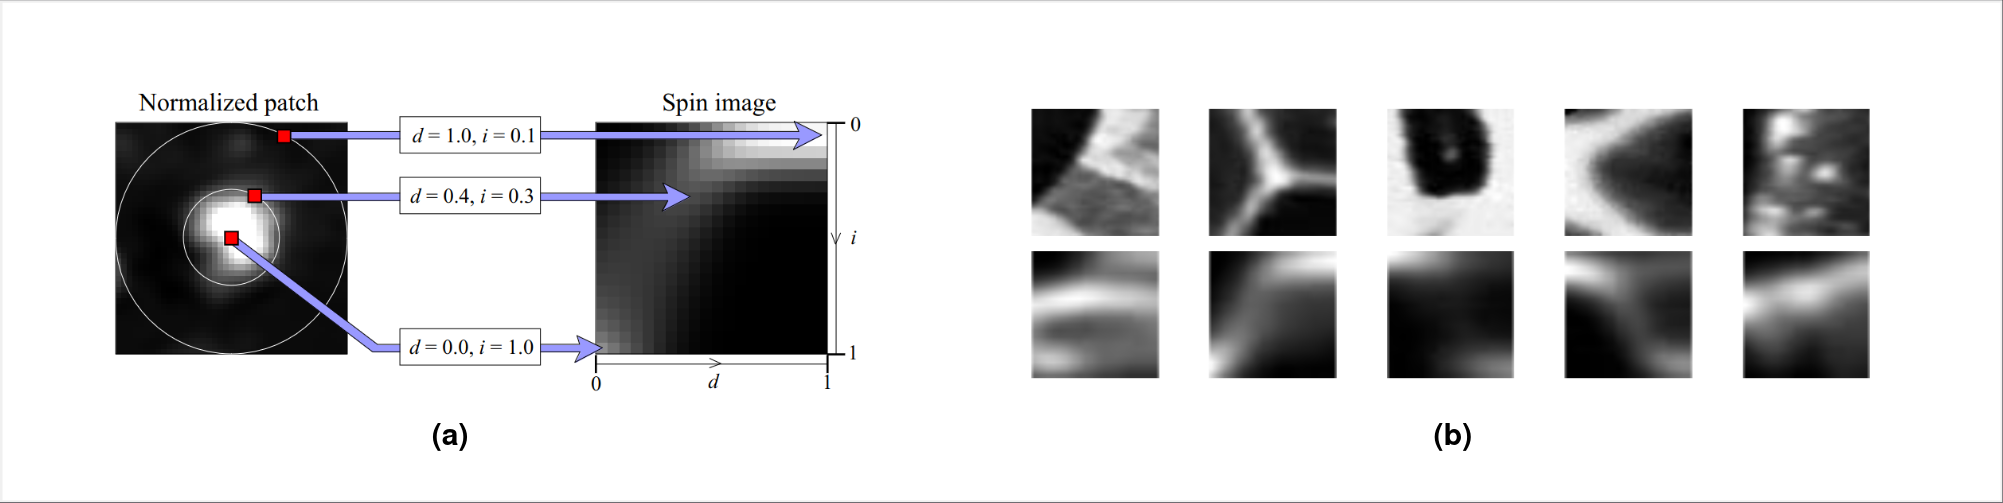
\includegraphics[width=\textwidth]{spin_image.png}
    \caption{\text{Spin} изображение: \textit{(a)} визуализация на съотнасяне между пиксел и кофа от хистограма; \textit{(b)} примерни \textit{spin} изображения; изображенията са собственост на \cite{spinimages}}
    \label{fig:spinim}
\end{figure}

\bigbreak

Подходът за изграждане на \textit{spin} изображения, избран в статия \cite{spinimages} не е перфектен. За всеки пиксел от нормализирания регион се обхожда всяка кофа от хистограмата. Следователно алгоритъмът е с висока времева сложност. При разпределение на приноса на пиксел с координати $\begin{bmatrix} d_0 \\ i_0 \end{bmatrix}$ към кофите от хистограмата се наблюдава, че колкото по-отдалечена е една кофа от $\begin{bmatrix} d_0 \\ i_0 \end{bmatrix}$, толкова по-малко принос получава тя. Съответно в някакъв момент той става неглижируем. Нашата разработка се преборва с този проблем, като прилага обхождане по ширина на матрицата на \textit{spin} изображението, започвайки от клетката с координати най-близки по Евклидово разстояние до $\begin{bmatrix} d_0 \\ i_0 \end{bmatrix}$. При обхождането за терминален връх се счита клетка $\begin{bmatrix} d \\ i \end{bmatrix}$, всички съседи, на която са обходени, или клетка $\begin{bmatrix} d \\ i \end{bmatrix}$, с принос $contrib_{d_0,i_0}(d, i) \leq \varepsilon, \varepsilon \in \mathbb{R}$.

\bigbreak

Друг проблем при предложения от \cite{spinimages} подход за изграждане на \textit{spin} изображения е свързан с наличието на дисбаланс в $d$ оста на изображения. Нека разглеждаме окръжности $O_0$ и $O_1$, съответно с радиуси $r_0$ и $r_1$, такива че $r_0 > r_1$. Очевидно периметъра на $O_0$ е по-голям от този на $O_1$. Това се наблюдава и в алгоритъма за изграждане на \cite{spinimages} изображения. Както споменахме, един нормализиран регион може да се разглежда като множество от концентрични окръжности. Тези по-близо до центъра разполагат с по-малък периметър, съответно по-малко пиксели. Наличието на по-малко пиксели близо до центъра означава, че винаги клетките от \textit{spin} изображението с по-малки $d$ координати ще имат по-малки стойности. Начин да се контрира този проблем е, като се модифицира $contrib_{d_0,i_0}$ функцията. Предлагаме вариант, където $contrib'_{d_0,i_0}(d, i) = \exp(-(d-d_0)^2(2\pi(d_0+\varepsilon))/(2\alpha) - (i-i_0)^2/(2\beta))$. Идеята е, че броят клетки на дистанция $d_0$ от центъра на нормализирания регион расте със скоростта на увеличение на периметъра.

\bigbreak

Разполагайки с множество от \textit{spin} изображения (дескриптори) $H, |H|=K, H \in \mathbb{R}^n, n, K \in \mathbb{N},$ за едно изображение $Im$, следващата стъпка включва изграждането на сигнатура за $Im$. Сигнатура дефинираме като крайно множество от претеглени едномерни хистограми $S = \{<V_k, w_k> | V_k \in \mathbb{R}^n, k,n \in \mathbb{N} $ и $\sum_{j=1}^{|S|} w_j = 1 \}$. Една сигнатура може да има произволен брой елементи.

\bigbreak

Начинът за намиране на сигнатура, използван в \cite{spinimages} започва с агломеративно клъстетиране на \textit{spin} изображенията. Избрано е агломеративно клъстериране защото е трудно предварително да бъде определен броя на клъстерите. Нека намерените клъстери са $J$ на брой и обозначим клъстер с $Cluster_j, 1 \leq j \leq J, j \in \mathbb{N}$. Нека броят на \textit{spin} изображенията причислени към $Cluster_j$ обозначим с $|Cluster_j|$. Тогава причисляваме тегло $w_j$ към $Cluster_j$, такова че $w_j = \frac{|Cluster_j|}{|H|}$, където $|H|$ е броят на всички \textit{spin} изображения. След това за всеки клъстер $Cluster_j$ откриваме центъра или т.нар. медоид чрез формулата $Medoid_j = \frac{\sum_{H \in Cluster_j} H}{|Cluster_j|}$. Намерената сигнатура е $\{<Medoid_1, w_1>, <Medoid_2, w_2>, \cdots, <Medoid_J, w_J>\}$.

\bigbreak

Слабост на избрания подход е, че класическото агломеративно клъстериране не се справя с откриване на клъстери с форма различна от хиперсферична. За да се преборим с този проблем в нашето решение предлагаме използване на \textit{HDBSCAN} (виж \cite{hdbscan}).

\bigbreak

Задачата за откриване на подобни изображения включва предварително изграждане на база от сигнатурите на всички изображения, сред които търсим подобни на входно такова. Нека наречем изображенията в базата предварителни. За всяко предварително изображение се запаметява изображението, заедно с неговата сигнатура. Детайли относно персистентност на решението могат да бъдат открити в следващите секции. Имплементацията предоставя възможност за търсене на $n, n \in \mathbb{N}$, най-подобни изображения на дадено входно на база неговата сигнатура. Следователно трябва да намерим начин за сравнение между две сигнатури.

\bigbreak

Решението предложено в \cite{spinimages} разглежда адаптация на \textit{Earth Mover's Distance (EMD)} като метрика за сравнение между две сигнатури. Нека имаме две сигнатури, съотевтно $\{(\mathbf{m_i}, u_i)\}$ и $\{(\mathbf{n_j}, v_j)\}$. \textit{EMD} стойността между двете се намира използвайки $\frac{\sum_i \sum_j f_{ij} d(\mathbf{m_i}, \mathbf{n_j})}{\sum_i \sum_j f_{ij}}$, където $f_{ij}$ са потокови стойности (\textit{flow values}), намерени чрез решаване на проблем за линейно програмиране, и $d(\mathbf{m_i}, \mathbf{n_j})$ е земната дистанция (\textit{ground distance}) между медоидите $\mathbf{m_i}$ и $\mathbf{n_j}$. Статията не изпада в допълнителни детайли като реферира към \cite{metricfordistributionsforims} и \cite{imretrievalwithoutsegmentation} за насоки относно имплементация на \textit{EMD}.

\bigbreak

Методът \textit{EMD} е още познат като метрика на Васерщайн. В практиката тя най-често бива използвана за намиране на близост между две хистограми. Нека $\mathbf{m}$ и $\mathbf{n}$ са две едномерни хистограми с еднаква размерност. Най-лесният начин да разберем \textit{EMD} е като си въобразим, че стойностите на случайните променливи от $\mathbf{n}$ олицетворяват купчини с пръст, а тези на $\mathbf{m}$ олицетворяват дупки. Пръстта е равна по обем на дупките. Нека разгледаме случайна променлива $i$ от $\mathbf{n}$ и случайна променлива $j$ от $\mathbf{m}$. Цената за пренос на единица пръст от $i$ към $j$ е равна на $|i-j|$. Следователно цената за пренос на пръст между еднакви случайни променливи е $0$. Задачата е да се запълнят дупките с пръст за минимална цена. \textit{EMD} е равно на минималната цена. Налични са множество библиотеки предоставящи решения на \textit{EMD} в този конкретен сценарий. Илюстрация на \textit{EMD} може да бъде открита на фигура \ref{fig:emdandreduction}.

\bigbreak

Намиране на близост между сигнатури, директно прилагайки \textit{EMD} е възможно, чрез дефинирането на проблем за линейно програмиране. \cite{metricfordistributionsforims} и \cite{imretrievalwithoutsegmentation} предоставят идеи, как може да бъде постигнато това чрез редукция до задача за минимална цена на мрежови поток (\textit{minimum cost network flow problem}) (или т.нар. оптимален поток). Задача от такъв вид може да бъде решена чрез линейно програмиране. Стандартен метод е използването на симплекс метода, но както ще покажем по-късно той е неоптимален. За целта ще дефинираме негова специализация над задачи за намиране на оптимален мрежови поток, наречена мрежови симплекс метод (\textit{network simplex method}).

\bigbreak

Ще започнем с дефиницията на това, какво е \textbf{потокова мрежа} (\textit{flow network}). Потокова мрежа наричаме ориентиран граф, където всеки връх притежава \textbf{ресурс}, който се пренася до съседните върхове чрез ребра. Всяко ребро има \textbf{капацитет} над максималния брой единици ресурс, които може да пренесе, както и цена за пренос на единица ресурс. Пренесения ресурс от ребро още наричаме поток на реброто. При някои задачи се допуска този капацитет да бъде безкрайност. Често ребрата биват наричани арки. Ресурсът притежаван от даден връх може да бъде положителен или отрицателен. Може да си мислим, че положителна стойност на ресурс означава излишък на ресурс, а отрицателна - недостиг. Граф където сумата от ресурсите на всички върхове е $0$ се нарича \textbf{балансиран}. 

\bigbreak

Нека имаме граф $G(V, E)$, ресурсът на връх $v \in V$ обозначаваме чрез $supply(v)$ и цената за пренос на единица ресурс през ребро $(u, v) \in E$ чрез $d_{uv}$. Потокът пренесен върху ребро $uv: (u, v) \in E$, обозначаваме чрез $x_{uv}$. Решение на задача върху потокови мрежи наричаме разпределение на потока, такова че за всеки връх $v \in V$ е изпълнено $\sum_{w: (v, w) \in E} x_{vw} - \sum_{u: (u, v) \in E} x_{uv} = supply(v) \iff \sum_{w: (v, w) \in E} x_{vw} - \sum_{u: (u, v) \in E} x_{uv} - supply(v) = 0$. Задачите се различават по параметрите, които оптимизират. Например задачата за намиране на минимален мрежови поток търси разпределение на пренесения поток, такова че $\sum_{(u, v) \in E} d_{uv} x_{uv}$ е минимално. Задачите над потокови мрежи намират редица приложения - логистични задачи, пренос на енергия в затворена система, пренос на течности по тръби и други.

\bigbreak

Нека разгледаме как можем да интерпретираме сравнение между две хистограми чрез \textit{EMD} като задача за намиране на минимална цена в потокова мрежа. Нека $\mathbf{m}$ и $\mathbf{n}$ са нормирани дискретни едномерни хистограми със случайни величини $\{1, 2, \cdots, n\}, n \in \mathbb{N}$. Стойността на случайна величина $j$ от $\mathbf{m}$ означаваме чрез $\mathbf{m}(j)$. Аналогично за $\mathbf{n}$. Нека всяка случайна величина $j$ от $\mathbf{m}$ представим като връх $w_j \in V$ в потокова мрежа $G(V, E)$ с ресурс $supply(w_j) = \mathbf{m}(j)$. Случайна величина $i$ от $\mathbf{n}$ представяме като връх $u_i \in V$ в потокова мрежа $G(V, E)$ с ресурс $supply(u_i) = -\mathbf{n}(i)$. Понеже хистограмите са нормирани, получената потокова мрежа е балансирана. Нека цената за пренос на почва от случайна величина $j$ в $\mathbf{m}$ до случайна величина $i$ в $\mathbf{n}$ представим като ориентирано ребро $(w_j, u_i) \in E$, такова че цената му е $|i - j|$. По този начин сведохме входните данни на \textit{EMD} до потокова мрежа $G$. Може да се докаже, че решението на \textit{EMD} е еквивалентно на решение за минимимална цена в потокова мрежа $G$. Интересно наблюдение е, че $G$ е бипартитен граф, с ребра излизащи от множество $W, W \subset V$ и влизащи в множество $U, U \subset V$. Върховете от $W$ са асоциирани само със случайни величини от $\mathbf{m}$, а тези от $U$ - $\mathbf{n}$. Следователно $W$ представя хистограма $\mathbf{m}$, а $U$ - $\mathbf{n}$. Илюстрация на редукцията може да бъде намерена на фигура \ref{fig:emdandreduction}. Показахме, че \textit{EMD} е частен случай на задача за намиране на минимална цена в потокова мрежа.

\begin{figure}[ht]
    \centering
    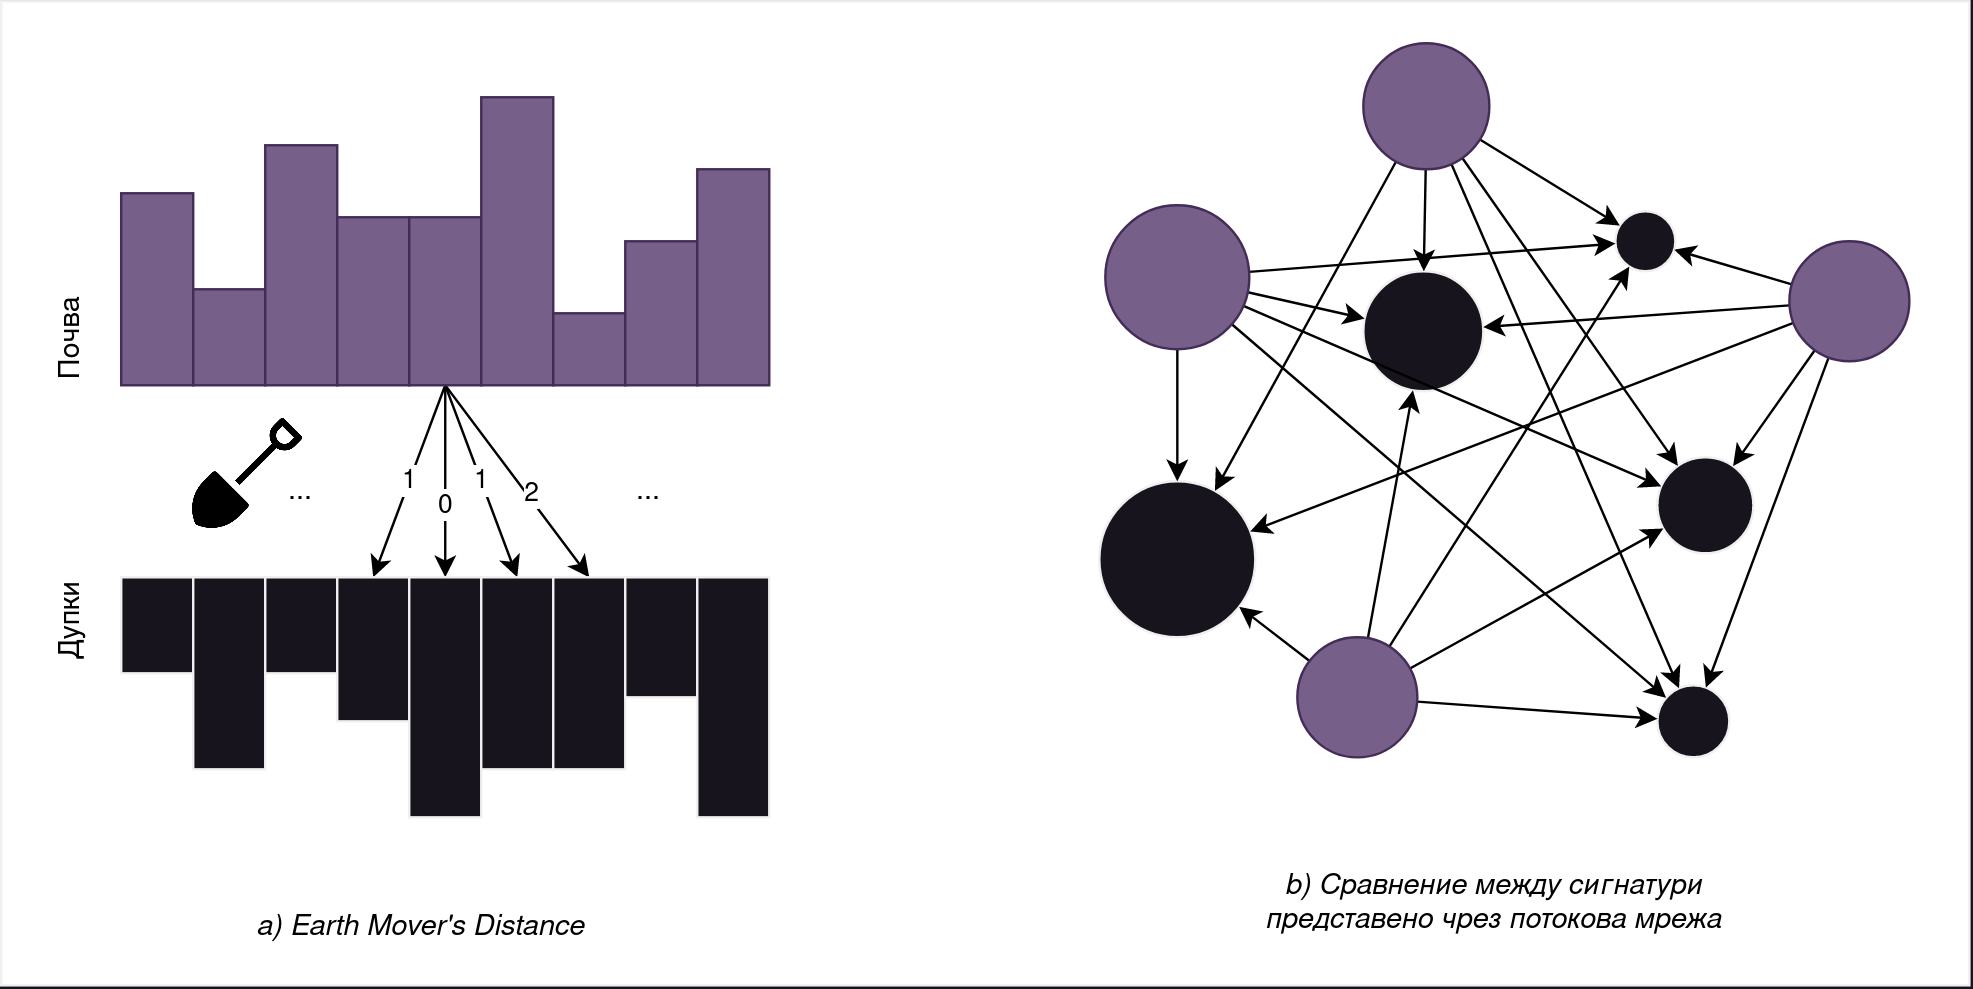
\includegraphics[width=\textwidth]{emd_and_reduction.png}
    \caption{\textit{(a)} \textit{Earth Mover's Distance (EMD)} приложен за сравнение на хистограми. Лилавите стълбчета са почвата, която трябва да бъде пренесена в черните дупки. Интерпретацията за физическа отдалеченост се имплементира посредством теглата на ребрата; \textit{(b)} Редукция на \textit{EMD} до задача за минимална цена на потокова мрежа. Лилавите върхове са почвата, която трябва да бъде пренесена в черните дупки. Радиусът на всеки връх илюстрира размера на неговия ресурс. Дължината на всяко ребро на фигурата илюстрира физическата дистанция между върховете.}
    \label{fig:emdandreduction}
\end{figure}

\bigbreak

Задачата за сравнение на две сигнатури $\mathbf{\alpha} = \{(\mathbf{med}_j, \mathbf{weight}_j)\}$ и $\mathbf{\beta} = \{(\mathbf{med}_i, \mathbf{weight}_i)\}$ не може да се редуцира до \textit{EMD} за сравнение на вектори с еднаква размерност, защото е възможно сигнатурите да са с различни кардиналности. Въпреки това е възможно да я редуцираме до задача за намиране на минимална цена в потокова мрежа използвайки похват подобен на този разгледан преди малко. Нека дефинираме потокова мрежа $G(V, E)$. За всяка двойка $(\mathbf{med}_j, \mathbf{weight}_j) \in \mathbf{\alpha}$ дефинираме връх $w_j \in V$ с ресурс $supply(w_j) = \mathbf{weight}_j$. За всяка двойка $(\mathbf{med}_i, \mathbf{weight}_i) \in \mathbf{beta}$ дефинираме връх $u_i \in V$ с ресурс $supply(u_i) = -\mathbf{weight}_i$. Понеже сумата от всички тегла асоциирани с медоиди в дадена сигнатура е нормирана (сумират се до $1$), получаваме, че $G$ е балансирана. Нека изберем случайно $(\mathbf{med}_j, \mathbf{weight}_j) \in \mathbf{\alpha}$ и $(\mathbf{med}_i, \mathbf{weight}_i) \in \mathbf{beta}$. Знаем, че векторите $\mathbf{med}_j$ и $\mathbf{med}_i$ са с една размерност. Следователно цената за пренос на ресурс от връх $w_j$ до връх $u_i$ представяме като ребро $(w_j, u_i) \in E$, такова че неговата цена е $\lVert \mathbf{med}_i - \mathbf{med}_j \rVert$. По този начин сведохме входните данни на задачата за намиране на близост между две сигнатури до потокова мрежа $G$. Може да се докаже, че намирането на минимална цена на потокова мрежа $G$ дава решението на \textit{EMD} за сравнение на вектори с различна размерност. Както преди, забелязваме, че $G$ е бипартитен, като можем да го разделим на две множества, съответно $W$ и $U$. Върховете от $W$ са асоциирани с елементи на $\mathbf{\alpha}$, а тези от $U$ - $\mathbf{\beta}$.  Илюстрация на редукцията може да бъде намерена на фигура \ref{fig:emdandreduction}.

\bigbreak

Задачата за намиране на минимална цена на потокова мрежа може да бъде сведена до система с ограничения. Тя може да бъде решена, използвайки метод за линейна оптимизация, като например симплекс (\textit{simplex}). Нека разполагаме с потокова мрежа $G(V, E)$ и използваме познатите ни до тук означения. Задачата за намиране на минимимална цена в $G$ се свежда до минимизиране на $\sum_{(u,v) \in E} d_{uv} x_{uv}$, такава че $\sum_{u: (u, v) \in E} x_{uv} - \sum_{w: (v, w) \in E} x_{vw} = -supply(v)$, $\forall v \in V$ и $x_{uv} \geq 0, \forall (u, v) \in E$. Нека $G$ е потоковата мрежа от фигура \ref{fig:flownet1}. Тогава минимизираме сумата $1 x_{ad} + 10 x_{ab} + 2 x_{db} + 4 x_{de} + 5 x_{ec}$, такава че:

\begin{equation}
    \label{eq:1}
    \begin{cases}
        -x_{ad} - x_{ab} = -5\\
        x_{ab} + x_{db} = 7\\
        x_{ec} = 2\\
        x_{ad} - x_{db} - x_{de} = -6\\
        x_{de} - x_{ec} = 2\\
        x_{uv} \geq 0, \forall (u, v) \in E
    \end{cases}.
\end{equation}

\begin{figure}[ht]
    \centering
    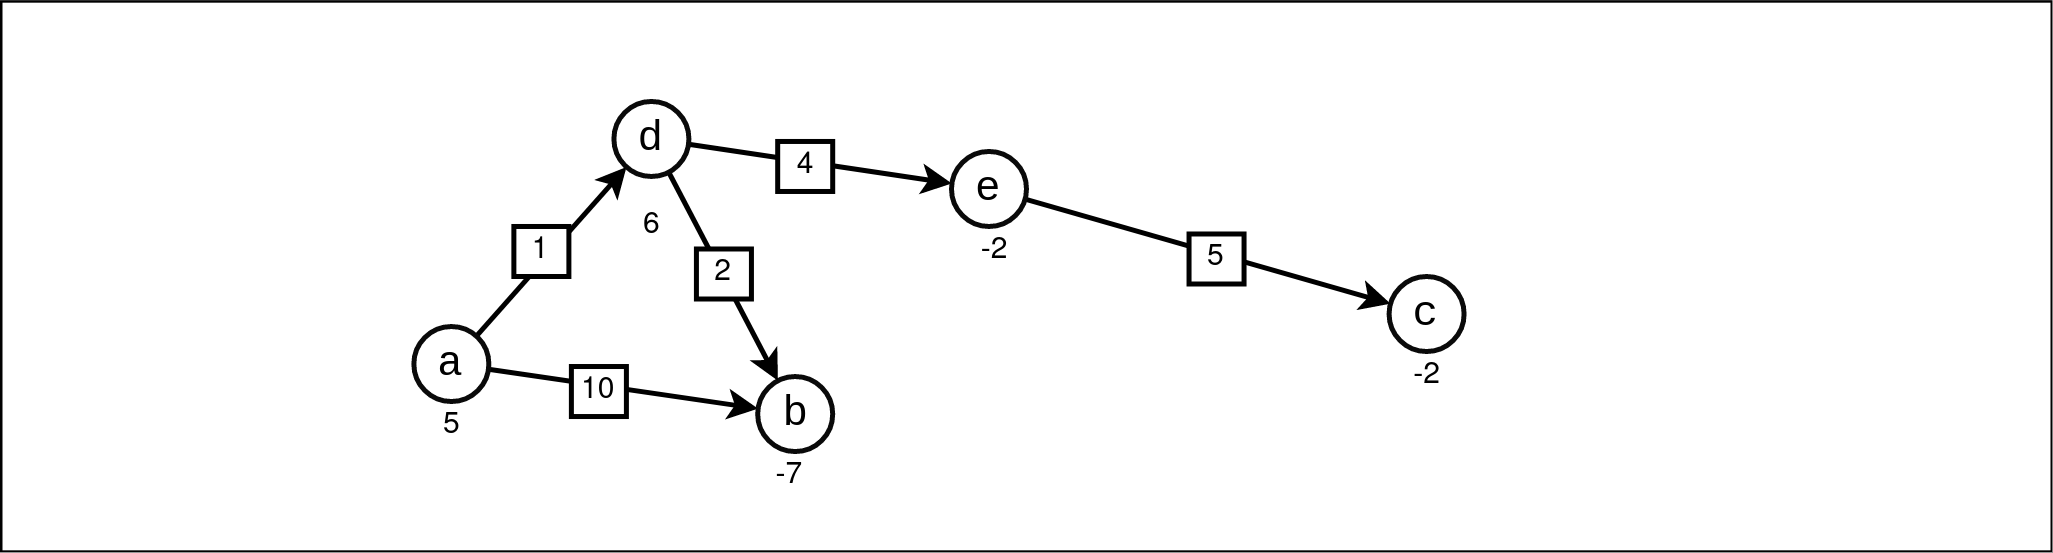
\includegraphics[width=\textwidth]{flownet1.png}
    \caption{\textit{Балансирана потокова мрежа, над която задачата за минимална цена на потока е решима. Ресурсът на всеки връх е написан под съответния връх. Цената за пренос на единица ресурс е написана в правоъгълниче на всяко ребро.}}
    \label{fig:flownet1}
\end{figure}

\bigbreak

Ще допуснем, че читателят е запознат със симплекс метода. За да можем да приложим симплекс метода, то трябва да преобразуваме система \ref{eq:1} до еквивалентна система с неравенства \ref{eq:2}:

\begin{equation}
    \label{eq:2}
    \begin{cases}
        -x_{ad} - x_{ab} \geq -5\\
        -x_{ad} - x_{ab} \leq -5\\
        x_{ab} + x_{db} \geq 7\\
        x_{ab} + x_{db} \leq 7\\
        x_{ec} \geq 2\\
        x_{ec} \leq 2\\
        x_{ad} - x_{db} - x_{de} \geq -6\\
        x_{ad} - x_{db} - x_{de} \leq -6\\
        x_{de} - x_{ec} \geq 2\\
        x_{de} - x_{ec} \leq 2\\
        x_{uv} \geq 0, \forall (u, v) \in E
    \end{cases}.
\end{equation}

\bigbreak

В получената система \ref{eq:2} има наличие на повече неравенства отколкото оптимизационни променливи, което води до ненужни свободни (\textit{slack}) оптимизационни променливи, което осезаемо увеличава извършената работа от страна на симплекс метода. Друго наблюдение е, че коефициентите пред всяка променлива са от множеството $\{-1, 0, 1\}$, съответно симплекс методът ще извърши още ненужна работа. Съществува оптимизация (частен случай) на симплекс метода, наречена мрежови симплекс (\textit{network simplex}), която ни позволява да се възползваме от система от вида на \ref{eq:1}, за да намалим времевата сложност на алгоритъма за линейно оптимиране.

\bigbreak

При ограничения от вида на \ref{eq:1}, съществува еквивалентно представяне на примитивите от стандартния симплекс метод чрез използване на графи. В тази статия ще разгледаме как методът работи, без да се впускаме в излишни детайли. Доказателството за това не е тривиално и разписването му изисква десетки страници. Читателят може да се обърне към \cite{networksimplexmethod} за пълните подробности и доказателство. Всички твърдения, които следват са спрямо система от вида на \ref{eq:1} и потокова мрежа $G(V, E)$.

\bigbreak

При решаване на стандартния симплекс метод се намират последователно решения на два вида системи. Едната система (тази от вида \ref{eq:1}) се нарича първична, а другата дуалната. Променливите от първичната система наричаме първични (\textit{primal variables}), а тези от дуалната са съответно дуални (\textit{dual variables}) и свободни (\textit{slack variables}). В статия \cite{networksimplexmethod} доказват, че първичните променливи съответстват на потока пренесен през дадено ребро. За да дефинираме знамението на дуалните и на свободните променливи в $G$ ще трябва да дефинираме какво означава базис в $G$.

\bigbreak

Решение, предоставено ни от симплекс метода се нарича базис, защото системите се представят като матрици. То е $n$-мерен вектор със стойности на първичните променливи. Казваме, че един базис не е първично недопустим (\textit{primal infeasible}) ако съществуват първични променливи, които са отрицателни. В противен случай е първично допустим. Аналогично казваме, че базисът е дуално недопустим (\textit{dual infeasible}) когато съществуват свободни променливи, които са отрицателни. В противен случай, той е дуално допустим. Базис е допустим ако той е едновременно първично и дуално допустим. Казваме, че един базис е оптимален когато той е допустим и минимизираното уравнение е с най-малката си възможна стойност при заместване на променливите (за \ref{eq:1} това е $min(1 x_{ad} + 10 x_{ab} + 2 x_{db} + 4 x_{de} + 5 x_{ec})$).

\bigbreak

Очевидно е, че променливите, които търсим са $x_{uv}: (u, v) \in E$). Имайки предвид, че базисите са винаги линейно-независими, в статия \cite{networksimplexmethod} доказват, че базисите са с размерност $|V|-1$. Казваме, че $G$ е слабо-свързан, когато $G$ е ориентиран и при заместване на всяко ребро в $G$ с ориентирано такова, новополученият граф $G'$ е свързан. Слабо-свързана компенента на $G$ наричаме свързана компонента от $G'$. Нека от тук нататък означаваме неориентираната версия на $G$ чрез $G'$. В статия \cite{networksimplexmethod} допускат, че $G$ винаги е слабо-свързан. В противен случай независимо се търси решение над всяка слабо-свързана компонента на $G$. В статия \cite{networksimplexmethod} доказват, че базис съответства на някое покриващо дърво в $G'$.

\bigbreak

От споменатото до тук, очевидно е, че ако базис $B$ е първично допустим, то потокът, течащ по ребрата от покриващото дърво $D$ съответстващо на $B$ е винаги неотрицателен. Статия \cite{networksimplexmethod} дава дефиниция на дуални променливи в $G$. На всяка дуална променлива $y_v$ съответства връх $v \in V$, като стойността на $y_v$ е минималната цена за достигане от корена на $D$ до $v$. Статия \cite{networksimplexmethod} дефинира свободна променлива $z_{uv}$, съответстваща на всяко ребро $(u, v) \in E$, като $z_{uv} = cost(u, v) + y_u - y_v$. Наличието на отрицателни свободни променливи, означава че дадено решение е дуално недопустимо, както и, че то е първично неоптимално.

\bigbreak

Нека $D(V, E_D)$ е покриващо дърво съответстващо на базис $B$. Изчисляването на потоковите променливи $x_{uv}: (u, v) \in E_D$ се осъществява чрез търсене в дълбочина. На всяко ниво на рекурсията, обхождаме обхождаме всяко ребро $(v, w) \in E_D$ излизащо от текущия връх $v \in V$. Напомняме, че $E_D$ е множество от неориентирани ребра, такова че $E_D \subseteq E'$, където $E'$ съдържа неориентирано ребро за всяко ориентирано от $E$. Ако $(v, w) \notin E$, то $x_{vw} = supply(w)$. В противен случай $x_{vw} = -supply(w)$. Модифицираме $supply(v) := supply(v) + supply(w)$. Продължаваме рекурсията.

\bigbreak

Както при стандартния симплекс метод намирането на оптимално решение се състои от започване със случаен базис (, който може да е недопустим) и двустъпков процес на въртене (\textit{pivoting}) на базиса. За целта статия \cite{networksimplexmethod} дефинира аналози на първично въртене (\textit{primal pivoting}) и дуално въртене (\textit{dual pivoting}).

\bigbreak

Нека започнем от случаен базис $B$, на който съответства покриващо дърво $D(V, E_D)$ на $G$. За да е възможно изпълнението на първично въртене е необходимо $B$ да бъде първично допустим, т.е. потокът $x_{uv}$ течащ по всяко ребро $(u, v) \in E_D$ да e неотрицателен, т.е. $x_{uv} \geq 0$. Процесът по първично въртене може да се обобщи чрез:

\begin{enumerate}
    \item Ако няма отрицателни свободни променливи $z_{uv} \le 0: (u, v) \in E_D$, то алгоритъмът приключва. В противен случай.
    \item Избираме случайно ребро $(u, v) \notin E_D$. Добра евристика е да изберем $(u, v)$ с най-малката свободна променлива $z_{uv}$.
    \item Добавяме случайно избраното ребро $(u, v)$ в $E_D$, при което се оформя цикъл $C$.
    \item Откриваме всички ребра от $C$, които са посока противоположна на $(u, v)$. Ако няма такива и общата сума от цените ребрата в цикъла е отрицателна, то знаем, че алгоритъмът за намиране на минимална цена няма край, защото няма оптимален базис (виж фигура \ref{fig:primalpivotcycle}). Интуицията зад безкрайната оптимизация е, че отрицателната цена на ребро може да зачитаме като печалба. Съответно е възможно ресурс да бъде пратен от $u$ и той да се върне в $u$ през ребрата от $C$, като по този начин $u$ е на печалба. Това може да се повтаря до безкрай.
    \item Избираме реброто $(p, q) \in E_D$ с най-ниската цена, което е срещуположно на $(u, v)$.
    \item Премахваме $(p, q)$ от $E_D$. Ако ребро $(a, b)$ е с посока обратна на $(u, v)$, то $x_{ab} := x_{ab} - x_{pq}$. Ако ребро $(a, b)$ е с посока тази на $(u, v)$, то $x_{ab} := x_{ab} + x_{pq}$. Очевидно $x_{uv} := x_{pq}$ и $x_{pq} := 0$ и вече няма цикъл. Доказателството за коректността на тази промяна може да бъде открито в статия \cite{networksimplexmethod}. Причината да премахнем реброто с най-ниска цена е за да запазим първичната допустимост на базиса (не бива да има отрицателни първични променливи).
    \item Преизчисляваме първичните, дуалните и свободните променливи.
\end{enumerate}

\begin{figure}[ht]
    \centering
    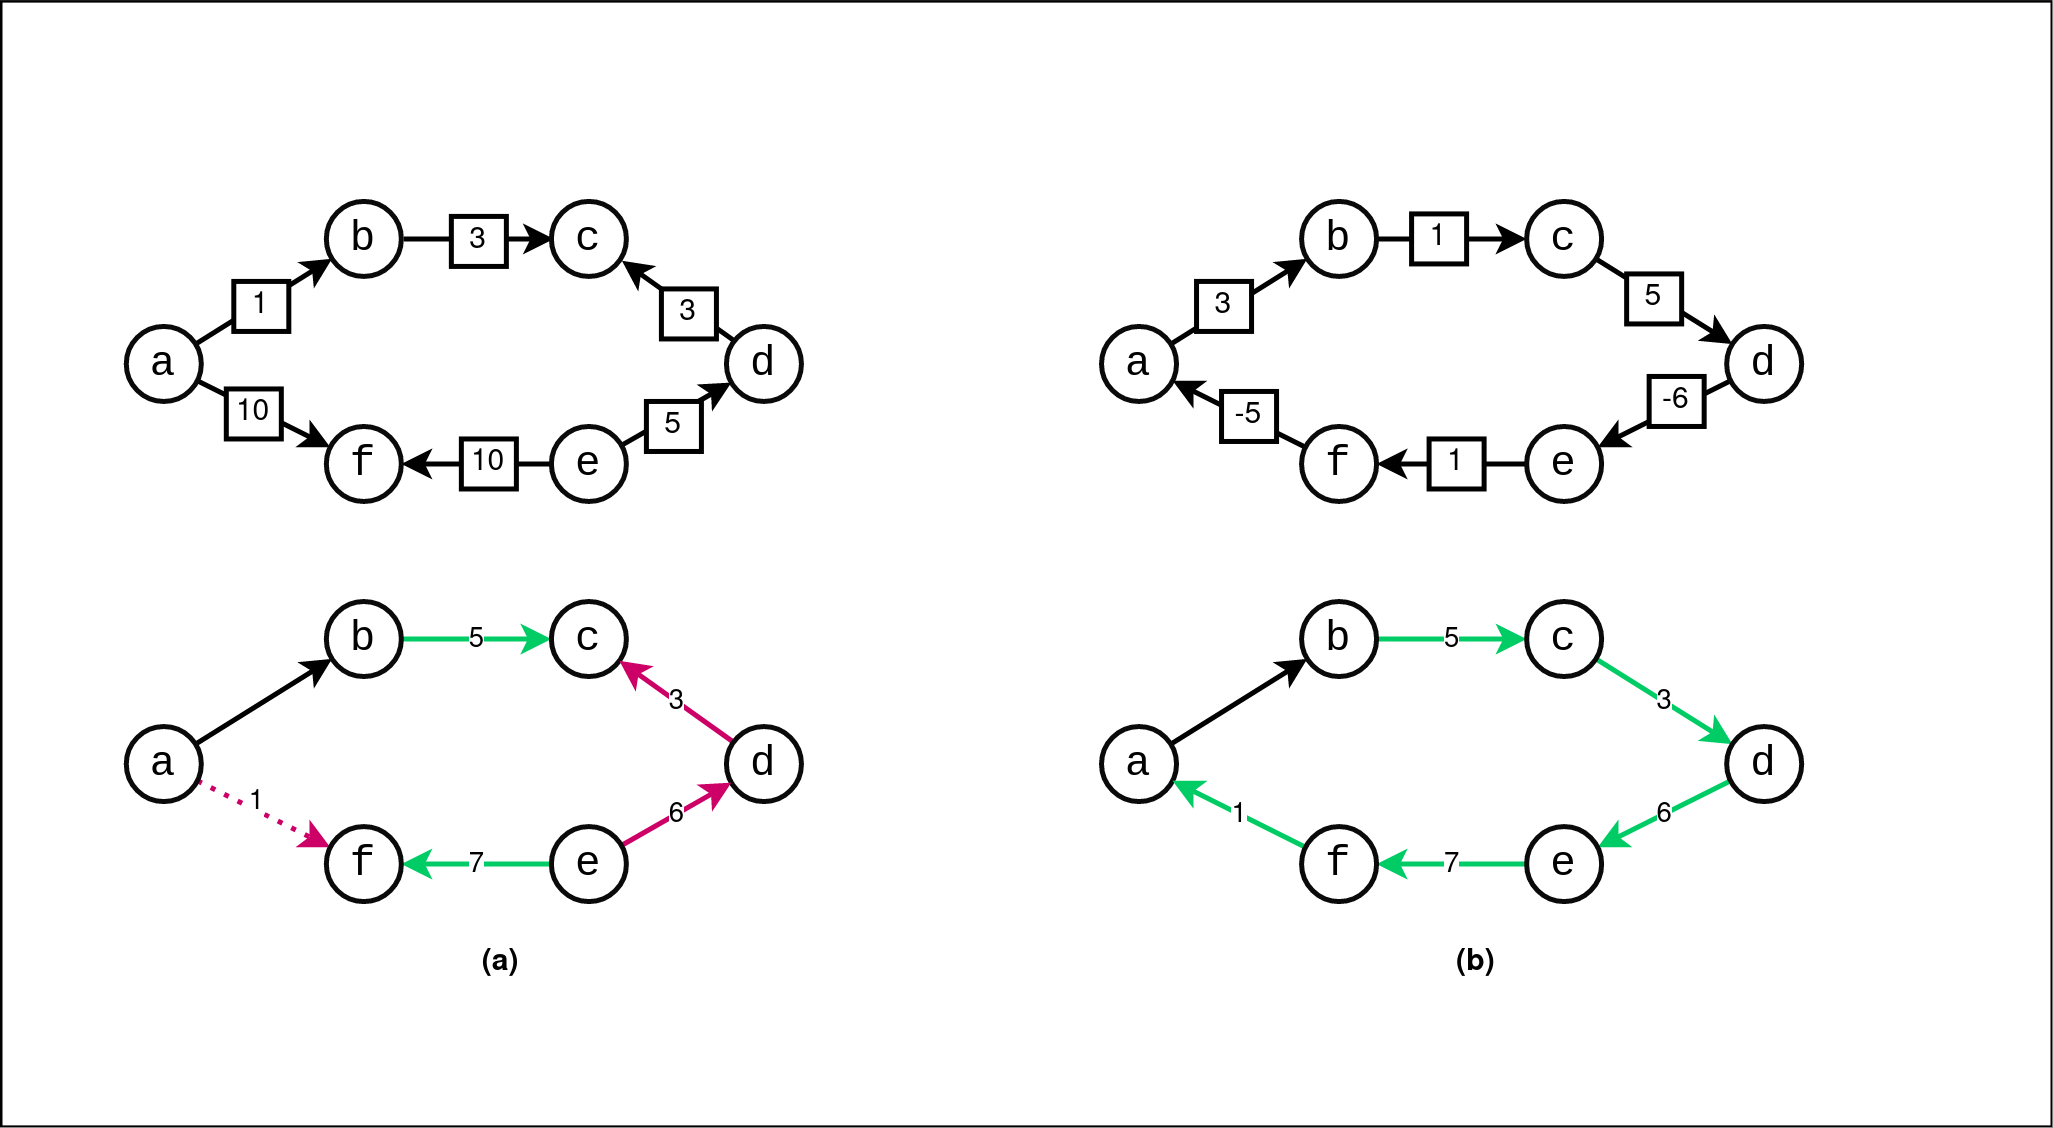
\includegraphics[width=\textwidth]{primalpivotcycle.png}
    \caption{\textit{Цикли образувани при първично въртене. Графите отгоре са подмножества от входните потокови мрежи. Графите отдолу са междинен резултат от изпълнението на алгоритъма. Над всяко ребро с цифра е надписан пренесения ресурс. Черното ребро е добавеното. Зелените ребра са с посока, тази на добавеното, а червените с обратна. Пунктирното червено ребро е това, което премахваме от базиса. (a) Цикъл, където ребрата са с положителна цена и има ребра в обратна посока. (b) Цикъл, при който откриваме, че задачата за оптимизация е неограничена.}}
    \label{fig:primalpivotcycle}
\end{figure}

\bigbreak

Преди да продължим трябва да докажем, че съществува оптимално първично решение при задачата за сравнение на сигнатури. Както споменахме след редукция на задачата за сравнение на сигнатури получаваме ориентиран бипартитен граф $G(V, E)$, където върховете могат да бъдат разделени на две множества, съответно $U$ и $W$, където $U \cap V = \emptyset$ и $U \cup W = V$. Всички ребра са от вида $(u, w) \in E: u \in U, w \in W$. Нека имаме покриващо дърво $D(V, E_D)$ над слабосвързания граф $G$. Очевидно е, че всички пътища в $G$ са от вида $v_0, \cdots, v_n$, където $(v_i, v_{i+1})$ е с различна посока от тази на $(v_{i+1}, v_{i+2})$, за $0 \leq i < i+2 \leq n$. Съответно е невъзможно наличието на цикъл с ребра от еднаква посока. Доказахме, че съществува оптимален базис получен след първично въртене над $G$. Доказателството е илюстрирано на фигура \ref{fig:primalboundednessproof}.

\begin{figure}[ht]
    \centering
    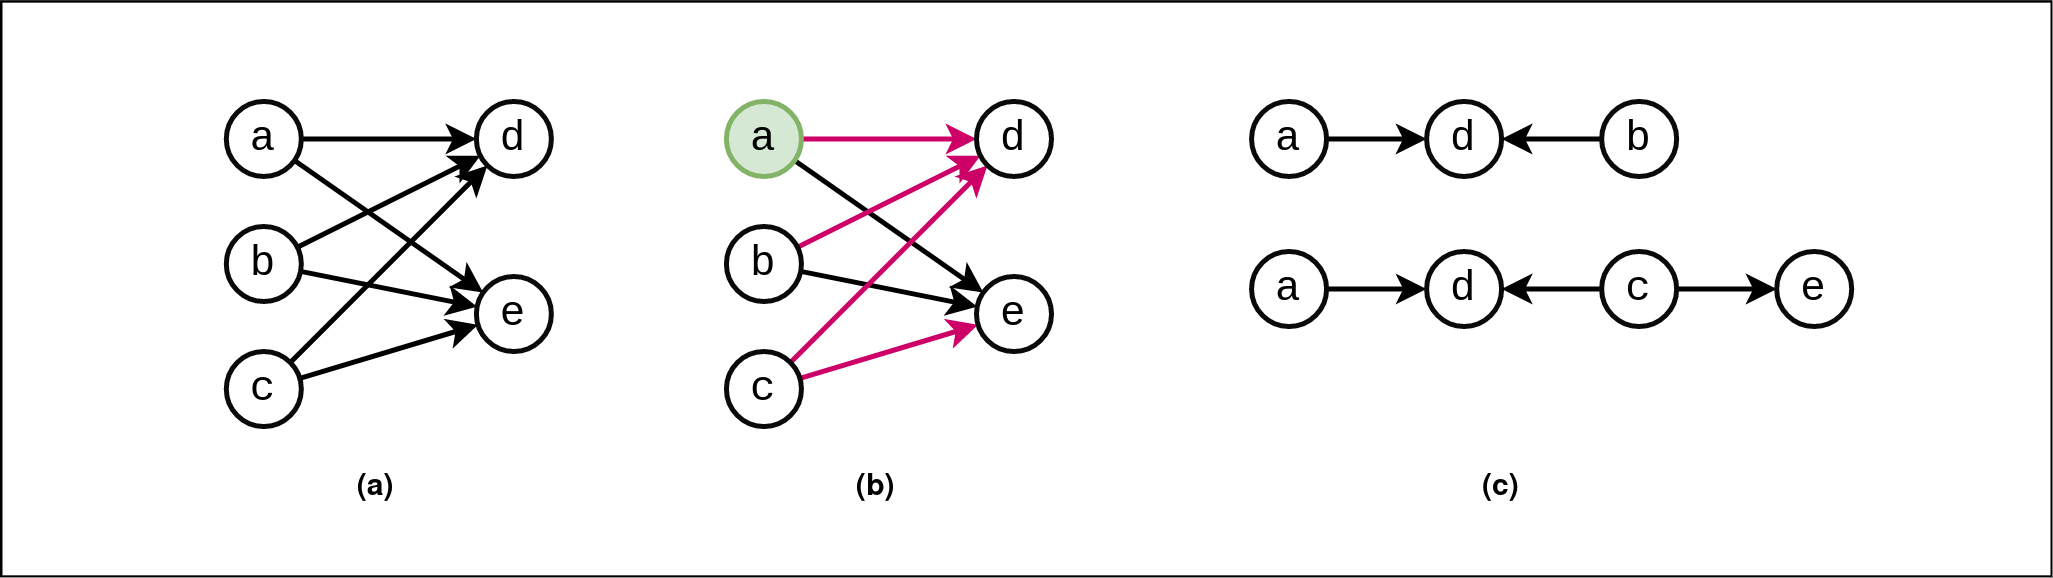
\includegraphics[width=\textwidth]{primalboundednessproof.png}
    \caption{\textit{(a) примерна потокова мрежа получена при сравнение на две сигнатури. (b) покриващо дърво с корен връх \textbf{a}. (c) всички пътища в покриващото дърво. Забелязваме как се редуват срещуположни ребра.}}
    \label{fig:primalboundednessproof}
\end{figure}

\bigbreak

Нека използваме същата нотация, както при първично въртене. Почваме от случаен базис $B$, на който съответства покриващо дърво $D(V, E_D)$ на $G$. За да е възможно дуално въртене е необходимо $B$ да бъде дуално допустим, т.е. да няма свободни променливи $z_{uv}, (u, v) \in E_D$, такива че $z_{uv} < 0$. Процесът по дуално въртене може да се обобщи чрез:

\begin{enumerate}
    \item Ако няма отрицателни първични променливи $x_{uv}, (u, v) \in E_D$, то алгоритъмът приключва. В противен случай.
    \item Избираме случайно ребро $(u, v) \in E_D$, такова че $x_{uv} < 0$. Добра евристика е винаги да избираме реброто с най-малка първична променлива.
    \item Премахваме реброто $(u, v)$ от $D$. Съответно останалите ребра от $D$ оформят две свързани компоненти. Нека компонентата, където се намира корена на $D$ означим с $C_0$, а другата с $C_1$.
    \item Търсим ориентирани ребра от вида $(a, b) \in E$, такива че те са противоположни на $(u, v)$. За ново ребро избираме това, което е противоположно на премахнатото и е с най-малка свободна променлива. Ако не съществуват ребра в противоположна посока на премахнатото, то задачата за оптимизация на минималната цена на потоковата мрежа е безкрайна и съответно алгоритъмът няма да приключи работа.
    \item Преизчисляваме първичните, дуалните и свободните променливи.
\end{enumerate}

\begin{figure}[ht]
    \centering
    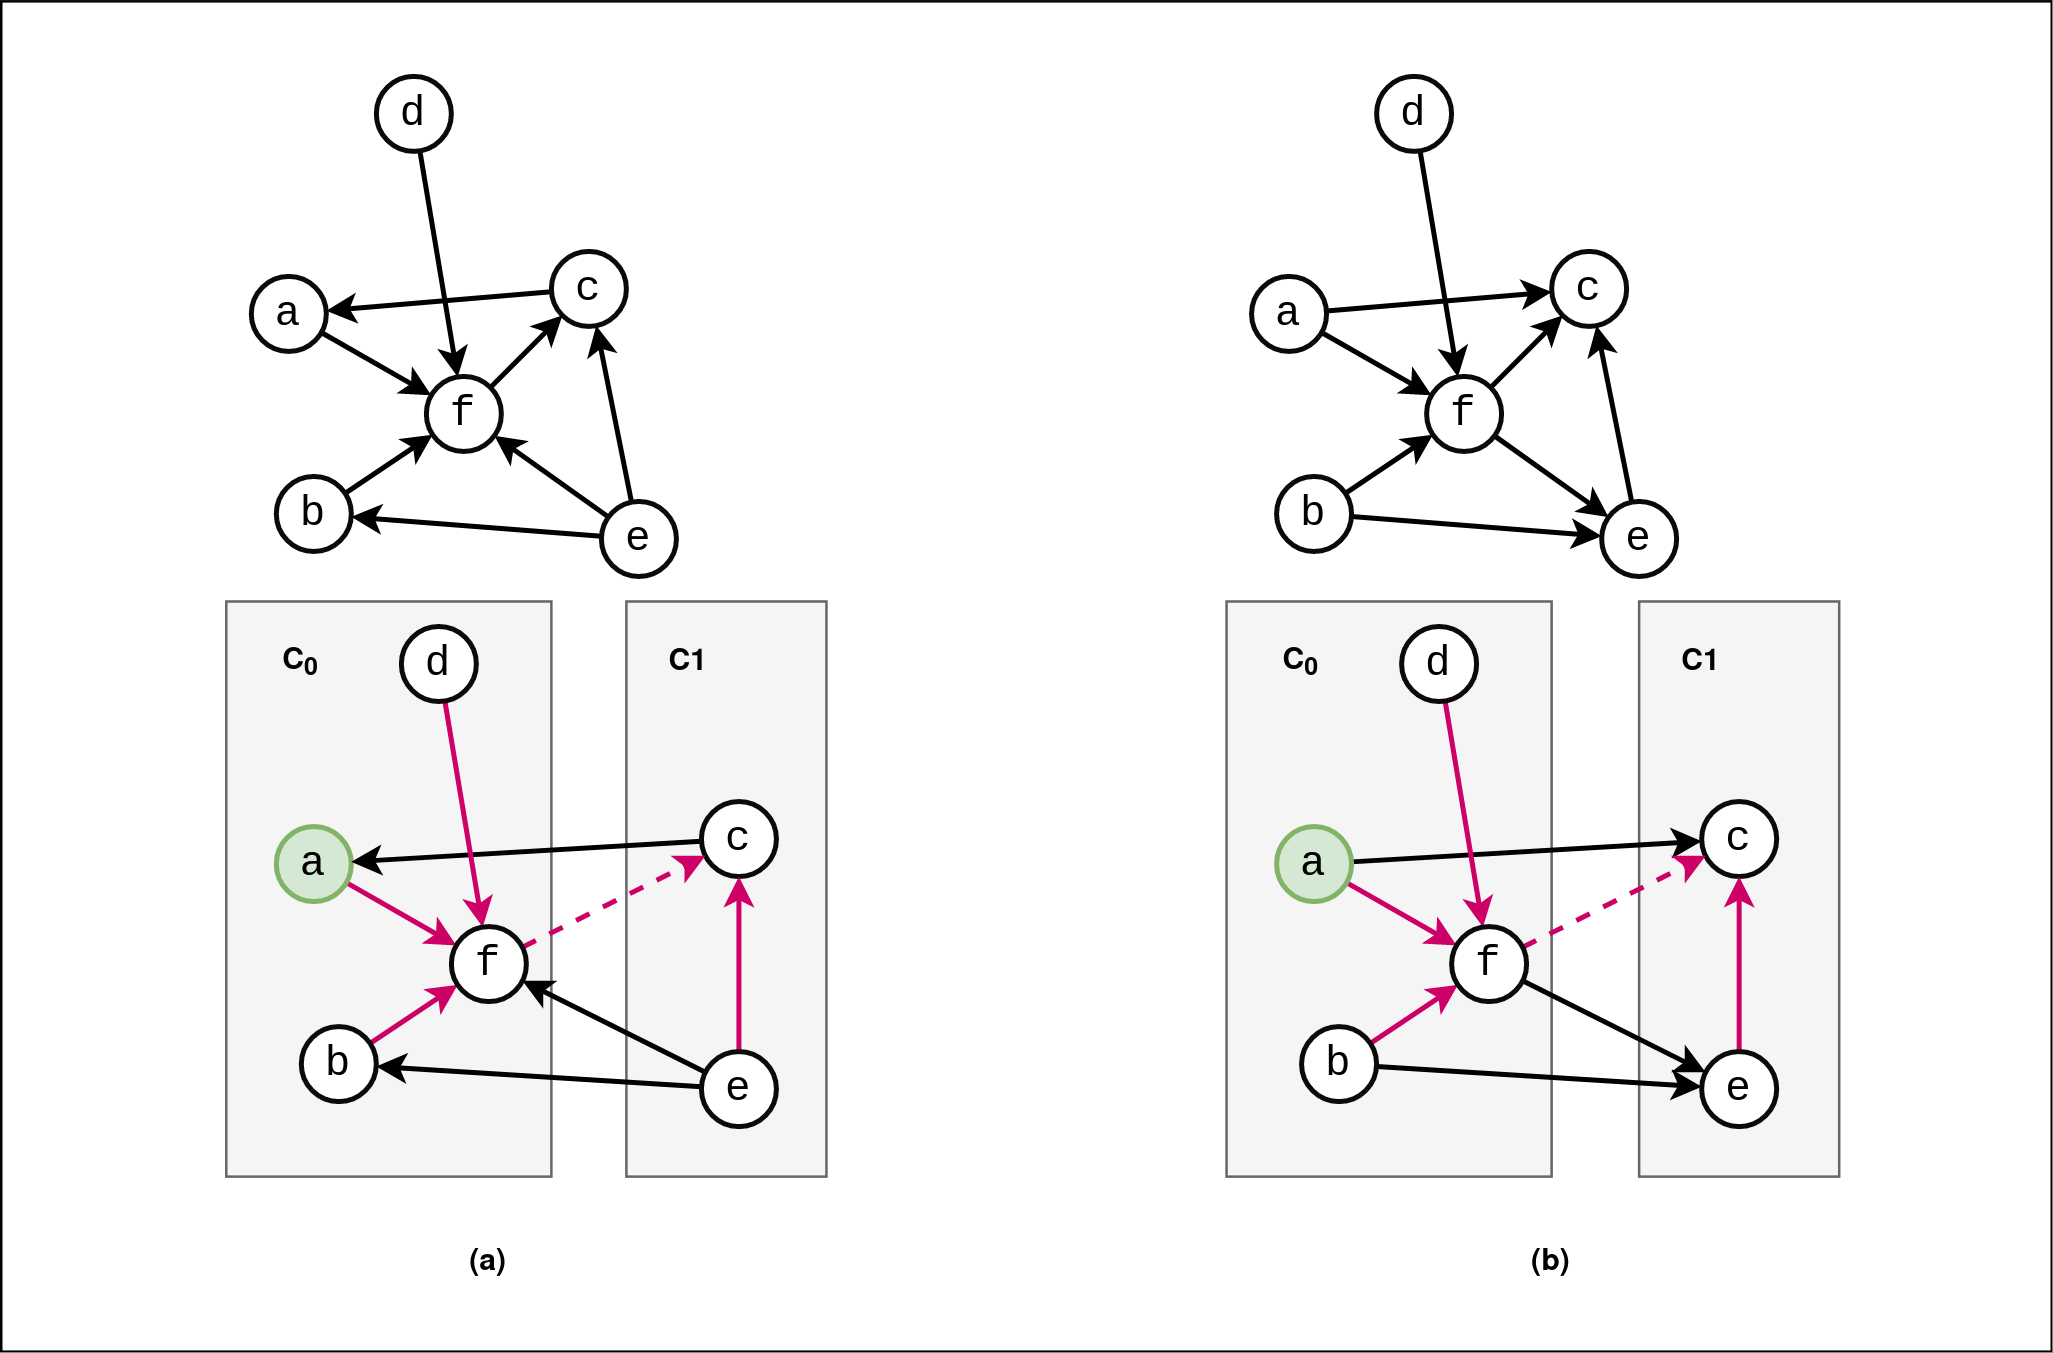
\includegraphics[width=\textwidth]{dualpivotsets.png}
    \caption{\textit{Прилагане на дуално въртене. Графите отгоре са входните потокови мрежи. Графите отдолу са междинен резултат от изпълнението на алгоритъма. Червените ребра представят ребрата от покриващото дърво. Корените на дърветата са отбелязани със зелено. С пунктирни линии са отбелязани премахнатите ребра. (a) Ситуация, при която е възможно алгоритъмът да има решение. (b) Ситуация, при която оптимизацията е безкрайна и алгоритъмът не приключва работа.}}
    \label{fig:dualpivotsets}
\end{figure}

\bigbreak

Преди да продължим трябва да докажем, че съществува оптимално дуално решение при задачата за сравнение на сигнатури. Както споменахме след редукция на задачата за сравнение на сигнатури получаваме ориентиран бипартитен граф $G(V, E)$, където върховете могат да бъдат разделени на две множества, съответно $U$ и $W$, където $U \cap V = \emptyset$ и $U \cup W = V$. Всички ребра са от вида $(u, w) \in E: u \in U, w \in W$. Нека имаме покриващо дърво $D(V, E_D)$ над слабосвързания граф $G$. При премахване на ребро е възможно да изпаднем в 4 ситуации спрямо размерите на $C_0$ и $C_1$. Първата ситуация е когато $C_0$ и $C_1$ са с поне два върха. Тогава е очевидно, че съществува ребро в обратната посока на премахнатото. Не е възможно $C_1$ да е само с 1 връх, защото ребрата непосредствено преди листа в покриващото дърво са винаги с положителни първични променливи. Нека имаме ребро $(u, v) \in E_D$. Ако $supply(v) \geq 0$, то реброто излиза от $v$ и влиза в $u$. Следователно $x_{uv} \geq 0$. Ако $supply(v) \leq 0$, то реброто влиза във $v$ и излиза от $u$. Следователно $x_{uv} \geq 0$. Защото премахнатото ребро е винаги с отрицателна първична променлива, доказахме, че е невъзможно $C_0$ да е само с един връх. Щом $G$ е балансиран то, очевидно не е възможно $C_1$ да бъде само с един връх.

\bigbreak

Имайки процедури за оптимизиране на дуално допустими и първично допустими базиси, ни трябва начин как да оптимизираме базиси на случайни графи. Това се реализира чрез двустъпков процес. Ще го разгледаме когато първо се прилага дуално въртене, но е възможно първо да се приложи първично:

\begin{enumerate}
    \item Изграждаме граф $G'$, състоящ се от копие на $G$, където цената на всички ребра е 0. Следователно всички дуални и свободни променливи са равни на 0. Всеки базис от $G'$ е дуално допустим.
    \item Намираме случайно покриващо дърво $D'$ на $G'$.
    \item Прилагаме дуално въртене, докато не получим оптимално решение или не открием, че оптимизационната задача е безкрайна. Нека оптималния базис е $D''$.
    \item Според статия \cite{networksimplexmethod} открития базис $D''$ ще бъде първично оптимален и над $G$.
    \item Прилагаме първично въртене, докато не получим оптимално решение или не открием, че оптимизационната задача е безкрайна. Получения оптимален базис $D$ е решение на задачата за намиране на минимална цена в потоковата мрежа $G$.
\end{enumerate}


% #############################################################################################################
\subsubsection{Инвариантна към мащаби трансформация на атрибути в комбинация с k най-близки съседи}

Този метод се базира на статия \cite{sift}. Идеята е проста. Откриваме точки на интерес и ги кодираме в дескриптори, използвайки \textit{SIFT} (обяснен отдолу). Дескрипторите са $n$-мерни вектори от реални числа. Нека сравняваните изображения означим с $Im_A$ и $Im_B$, като търсим подобни изображения на $Im_A$, а $Im_B$ е част от базата с изображения. За $Im_A$ и $Im_B$ откриваме множества от \textit{SIFT} дескриптори, съответно $S_A$ и $S_B$. За всеки дескриптор от $S_A$ търсим най-близкия до него дескриптор $S_B$, използвайки алгоритъма за намиране на най-близък съсед. Обратно - за всеки дескриптор от $S_B$ търсим най-близък до него дескриптор от $S_A$, използвайки алгоритъма за намиране на най-близък съсед. Като метрика за близост използва норма, като например $L2$. Зачитаме съвпадение между дескриптор $v \in S_A$ и дескриптор $u \in S_B$, единствено ако най-близкия съсед на $v$ е $u$ и най-близкия съсед на $u$ е $v$. Следва филтрация, където премахваме двойки съвпадащи дескриптори, които са на дистанция по-голяма от $tresh \in \mathbb{R}$. Нека броят на дескрипторите с нефилтрирани съвпадения от $Im_A$ означим с $matchcount(Im_A)$. Казваме, че изображение $Im_B$ е подобно на/идентично с $Im_A$, ако $\frac{matchcount(Im_A)}{|S_A|} > \varepsilon$, където $0 \leq \varepsilon \leq 1$ играе ролята на праг.

\bigbreak

Инвариантна към мащаби трансформация на свойства (\textit{Scale Invariant Feature Transform (SIFT)}) е един от най-успешните подходи за откриване на точки на интерес. Те са инвариантни към скалиране, ротация, отместване и частично инвариантни към промяна на илюминация и локална дисторция.  Откритите точки на интерес се явяват като апроксимация на тези, открити от главната визуална кора на приматите по това, че споделят подобно кодиране на форми и цвят (виж \cite{primatevisualcortex}). SIFT е разделен на няколко стъпки - откриване на потенциални точки на интерес, тяхната филтрация и присвояване на съответно векторно представяне.

\bigbreak

За да се открият потенциалните точки на интерес в изображение $I$ се започва с изграждането на \textbf{пространство на мащабите}. Намират се $n$ на брой октави на $I$, където над всяка октава, $k+1$ пъти последователно е приложен Гаусов филтър. Приложеният филтър на стъпка $s$ е със стандартно отклонение $\sigma_s, 0 <= s < k+1, s \in \mathbb{N}$, където $\sigma_{s+1} = 1.6 \sigma_s$. За всяка октава $i$ намираме разликата между всеки две последователно Гаусови филтрирания $j$ и $j+1$ (т.нар. разлика между Гаусови филтрирания (\textit{Difference of Gaussians (DoG)})), където $i < n, j < k, i, j \in \mathbb{N}$. Съответно пространството на мащабите се състои от $nk$ на брой изображения (виж фиг.). Нека интензитетът на точка $(x, y)$ на изображението от $j$-тото ниво на $i$-тата октава означим като $I_{ij}(x,y)$.

\bigbreak

Получените изображения апроксимират прилагането на Лапласов оператор, при който изпъкват очертанията на фигурите. Друга аналогия, ако разглеждаме $I$ като сигнал, е тази с \textit{band-pass filter}, защото прилагането на Гаусов филтър премахва високите честоти, а $DoG$ премахва честотите от по-замъгленото изображение (т.е. ниските). С други думи всяко ниво от пространството на мащабите представя конкретен честотен интервал на входното изображение $I$. За всеки такъв интервал \textit{SIFT} открива екстремални точки, които са потенциални точки на интерес. Една точка $(x, y)$ от $I_{ij}$ наричаме екстремална, ако за интензитетът ѝ $I_{ij}(x, y)$ е изпълнено $I_{ij}(x, y) >= I_{(i+r)(j+p)}(x+n, y+m) \forall r,p,n,m \in \{-1, 0, 1\}$. Тогава ако релацията за съседство дефинирана над изображението е $8$-съседство, се правят $9+8+9=26$ сравнения (виж фиг.).

\bigbreak

Някои от откритите до тук екстремални точки е възможно да са нестабилни спрямо трансформации, съответно е желателно те да бъдат премахнати. За подобрена точност, при процеса на филтрация, сигнала на изображението се конвертира от дигитален в аналогов. Точната локация на всеки екстремум $p=(x, y)$ за изображение $I_{ij}$ се апроксимира чрез \textbf{развитие на Тейлър} с център на координатната система $(x, y, \sigma_j)$: \\

$D(\varphi) = D + \frac{\partial D^T}{\partial \varphi}\varphi + \frac{\varphi^T}{2}\frac{\partial^2 D}{\partial \varphi^2}\varphi$ \\

, където $\sigma_j$ е стандартното отклонение за $I_{ij}$ и $\varphi=(x_{offset},y_{offset},\sigma_{offset})^T$ е отместване спрямо центъра на координатната система. Отместването към аналоговия екстремум $\hat{\varphi}$ намираме чрез откриване на корените на $D'$. Ако $max(\lvert\hat{\varphi}\rvert) > 0.5$, то истинският екстремум е по-близо до друга точка на интерес. Следователно изчисляваме наново $D$ с център на координатната система $(x, y, \sigma_j) + \hat{\varphi}$ и повтаряме итеративно процеса. В противен случай приемаме, че отместването на екстремума е $\hat{\varphi}$.

\bigbreak

Ако един екстремум не е достатъчно изпъкнал, т.е. $D''(\hat{\varphi}) < 0.03$, то се предполага, че той е нестабилен. Следва елиминация на точки намиращи се върху ръбове, където се използват характеристичните стойности на Хесиановата матрица на $D$. Новата локация на точката на интерес след процеса на филтрация е $(x, y, \sigma_j) + \hat{\varphi}$.

\bigbreak

Предните стъпки подсигуряват инвариантност към отместване и скалиране. Чрез тази стъпка се постига инвариантност към ротация на изображението. За дадена точка на интерес $(x, y)$ от октава $i$ със стандартно отклонение $\sigma$ наричаме съответното Гаусово филтриране $I_{\sigma}$. В околност около $(x, y)$ намираме размера и ориентацията на всеки градиент: \\

$m(x', y') = \sqrt{(I_{\sigma}(x'+1,y') - I_{\sigma}(x'-1,y'))^2 + (I_{\sigma}(x', y'+1) - I_{\sigma}(x', y'-1))^2}$ \\
$\theta(x', y') = \arctan(I_{\sigma}(x',y'+1) - I_{\sigma}(x',y'-1), I_{\sigma}(x'+1,y') - I_{\sigma}(x'-1, y'))$ \\

Създава се хистограма с 36 кофи, всяка съответстваща на интервал от $10\degree$. Всяка точка $(x', y')$ от околността $(x, y)$ се причислява към конкретна кофа според ориентацията си, като добавената стойността се претегля според магнитута и стандартното отклонение. Намира се теглото на най-тежката кофа, като оцеляват само кофите с тегло поне $0.8$ от теглото на най-тежката кофа. За всяка оцеляла кофа се създава ключова точка с тази ориентация.

\bigbreak

За изграждането на финалния дескриптор на точка на интерес се взима регион с размер $16 \times 16$ около нея. Той се разбива на 16 подрегиона, всеки с размер $4 \times 4$. За всеки регион се създава хистограма с 8 кофи. Съответно всеки дескриптор на точка на интерес има размерност $16 \times 8 = 128$. Подобно на предната стъпка, за всяка точка от този регион се намира ориентация и магнитут. За инвариантност на ротацията и отместването се използват координатната система на точката на интерес, чиито дескриптор се пресмята. За добавена инвариантност към илюминация се извършва нормализация и подрязване на финалния дескриптор.


% *************************************************************************************************************
\subsection{Архитектура и системен дизайн}

Решението може да се използва под формата на \textit{HTTP} сървър с прагматичен \textit{REST} интерфейс. Избрано е името на сървъра да е \textit{Livy}, по името на римския историк Титус Ливиус. Интерфейсът позволява изпълнението на основните 3 функции при задачата за откриване на най-подобни/идентични изображения. Те са добавяне на ново изображение в базата от изображения, търсене на идентификатори на топ $n, n \in \mathbb{N}$ най-подобни/идентични изображения и извличане на изображение по идентификатор. Употребата на \textit{REST} интерфейса е опростена чрез добавянето на максимално опростен потребителски интерфейс. Съответно имаме наличието на класическа трислойна архитектура. Виж фиг. \ref{fig:sequencediagrams}.

\begin{figure}[ht]
    \centering
    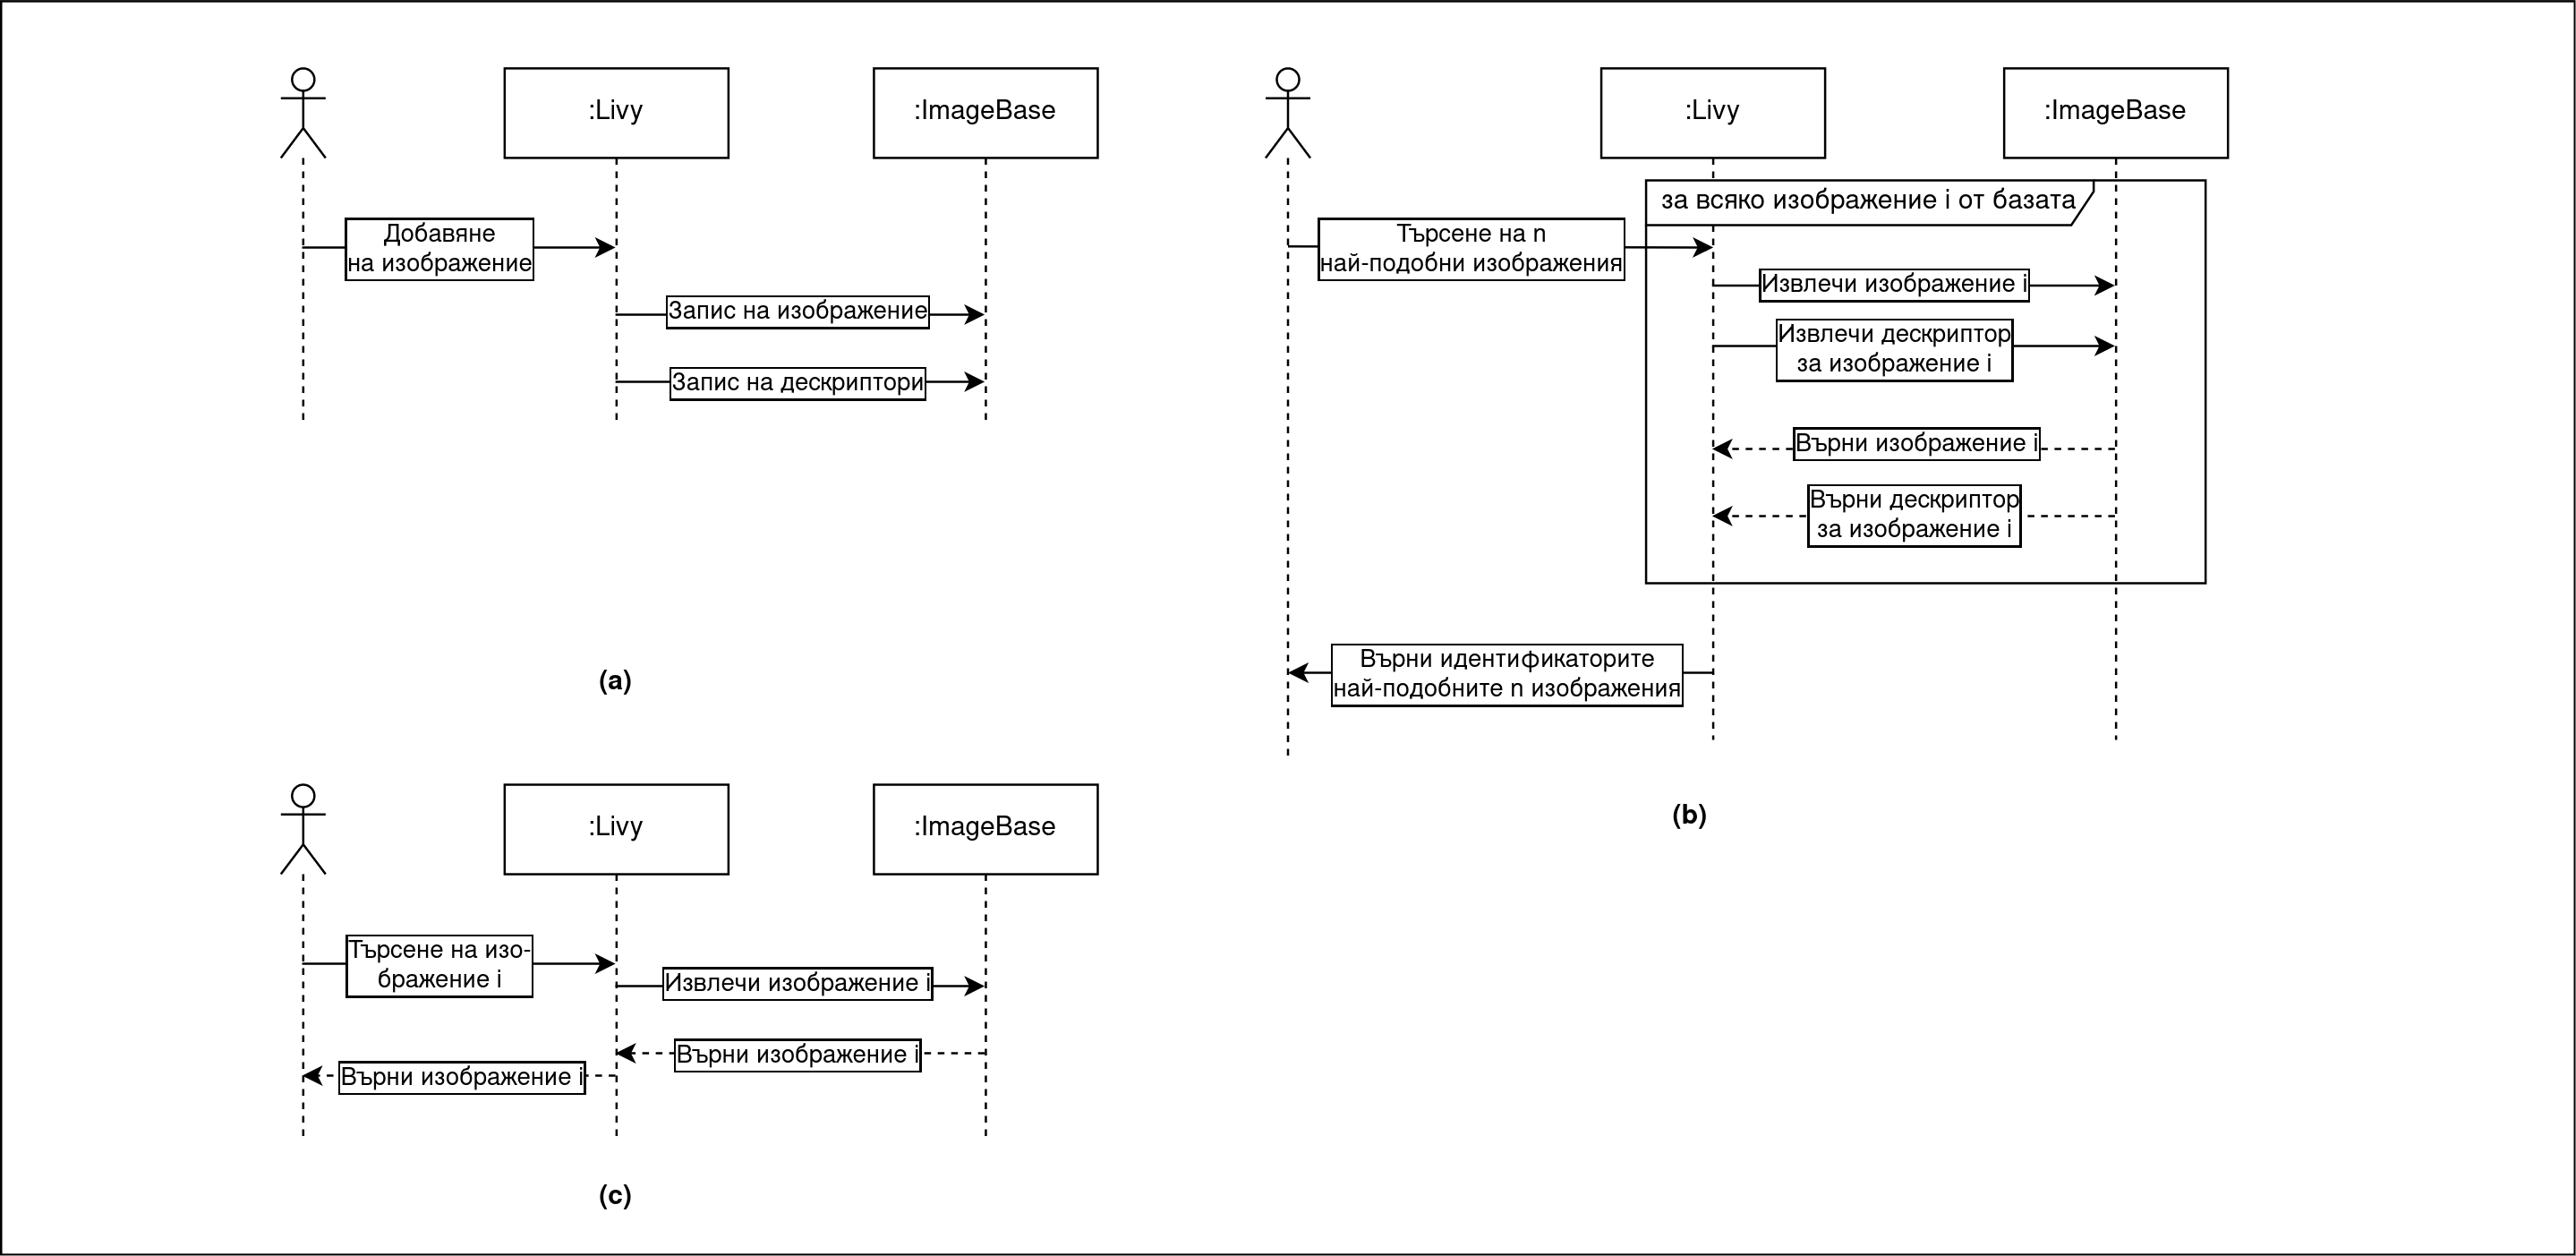
\includegraphics[width=\textwidth]{sequencediagrams.png}
    \caption{Сценарии за употреба на \textit{livy}: \textit{(a)} Добавяне на изображение; \textit{(b)} Търсене на $n, n \in \mathbb{N}$ най-подобни/идентични изображения на входно такова; \textit{(c)} Извличане на изображение по идентификатор от базата с изображения;}
    \label{fig:sequencediagrams}
\end{figure}

\bigbreak

При изграждането на системния дизайн са спазени принципите на чиста архитектура (\textit{Clean architecture}) въведени от книгата \cite{cleanarchitecture}. Съществува ясно разделение между контролери, хранилища, услуги и модели. От структурата на директориите отдолу се забелязва, че методите за решаване на задачата задачата са имплементирани в отделни услуги, съответно \textit{siftknn.py} и \textit{signature.py}. Имплементацията на мрежовия симплекс метод може да бъде открита под пакета \textit{livy/livy/dedup/model}. \textit{REST} интерфейса е имплементиран под \textit{livy/livy/api}. Сървърът може да бъде стартиран посредством \textit{make setup \&\& . .venv/bin/activate \&\& make serve}.

\begin{lstlisting}[language={}, caption={Описание на директорийната структура на имплементацията}]
livy/
|--cmd/
   |--server/
      |--main.py # main entry point
|--livy/ # internal livy library
   |--api # HTTP request handlers
      |--dedup.py # Deduplication request handlers
   |--dedup
      |--feature
         |--sift.py # SIFT feature extractor implementation.
         |--spin.py # Spin image extractor implementation.
      |--model # models and algorithms over them as known in clean architecture. Covers network simplex.
         |--dual.py # Dual variable calculation functions.
         |--dualpivot.py # Dual pivoting procedure functions.
         |--flow.py # Flow variable calculation functions.
         |--graph.py # Flow network common structures.
         |--networksimplex.py # A function that runs the whole network-simplex method.
         |--primalpivot.py # Primal pivoting procedure functions.
         |--spanningtree.py # A function to find a spanning tree (aka basis) of a flow network.
         |--state.py # Contains common networksimplex result structures.
      |--service # service objects
         |--service.py # common service definition.
         |--siftknn.py # sift + kNN approach.
         |--signature.py signature service definition.
      |--store # image store implementations.
   |--depinjection # dependency injection utilities used in HTTP handlers.
   |--id # package containing ID structure definitions.
   |--model # package containing common model definitions that are used everywhere.
|--tests
   |--subsystem # contains accuracy tests that are run against services.
   |--unit
|--web # UI
|--Makefile # Useful make targets for using the project.
\end{lstlisting}

% *************************************************************************************************************
\subsection{Използвани технологии}

Сървърната част е изградена предимно, използвайки програмния език \textit{python3}. За управление на зависимостите се използва \textit{pip3} в комбинация с виртуални среди. Често има повторение на използваните команди при разработка на проекта. По този повод е дефиниран \textit{Makefile} с множество от мишени (\textit{targets}), които могат да се изпълняват посредством \textit{make} командата. За обработка на изображения се използва библиотеката \textit{opencv}. За някои по-сложи математически операции се използва \textit{numpy}.

\bigbreak

Съществуват много библиотеки, които може да бъдат използвани за намиране на метрика на Васерщайн (напр. \textit{scikit-learn}), но решенията от тях са приложими единствено в опростения вариант разглеждан от фигура \ref{fig:emdandreduction} \textit{(a)}. Съществуват две публично-достъпни имплементации, удовлетворяващи случая описан от фигура \ref{fig:emdandreduction} \textit{(b)}. Една от тях е използваема единствено посредством \textit{python2}. Другата \textit{networkx} е написана за \textit{python3}, но не винаги намира решения, когато задачата за оптимизация на минимална цена на потоковата мрежа е решима. Съответно е направена имплементация на мрежовия симплекс метод.

\bigbreak

За изпълнение на тестовете се използва вградения в \textit{python3} пакет \textit{unittest}. Имплементацията на \textit{REST} интерфейса е направена посредством \textit{fastapi}, която предоставя имплементация сравнима по производителност с тази в по-оптимизирани езици като \textit{go}. Интерфейса е написан чрез \textit{css}, \textit{html} и \textit{javascript}.

% *************************************************************************************************************
\subsection{Eксперименти}

Целта на експериментите е да измерят емпирично каква е точността на разгледаните решения. Те са имплементирани под формата на тестове, намиращи се на ниво подсистема (\textit{subsystem tests}). За измерване на точност на задачата за откриване на най-близките $n, n \in \mathbb{N}$ най-подобни/идентични изображения се дефинира следния тестови сценарий - зареждаме база от изображения с всички изображения от множесто $S$. В последствие правим извадка на $k$ на брой случайни изображения от $S$, върху които извършваме трансформации (напр. афинни). Нека множеството на трансформираните изображения означим с $S'$. Съществува инекция $f$ на изображенията от $S'$ към изображенията $S$, такава че $f(s') = s, s' \in S', s \in S$. За всяко изображение $s' \in S'$ търсим най-близките $n, n \in \mathbb{N}$ изображения от $S$ използвайки имплементация на конкретен метод за решаване на задачата за намиране на най-подобни/идентични изображения. Нека за това дефинираме функцията $top(n, s'), s' \in S'$, множество $K \subset S$, такова че $|K| = n$, т.е. $top$ връща най-подобните $n$ изображения от $S$. Нека ако $f(s') \in top(n, s')$ за $s' \in S'$, то $success(n, s') = 1$, в противен случай $success(n, s') = 0$. Метриката за точност на алгоритъма дефинираме като $\frac{\sum_{s' \in S'} success(n, s')}{|S'|}$. Възможен начин за параметризиране е чрез подаване на различни стойности на $n$, както и на различни параметри на трансформациите прилагани над изображенията. Виж таблица \ref{table:1} за резултати. Тестовете са направени над множеството от данни \textit{COCO 2017}. От тестовете научаваме, че колкото и да е интересен методът на сигнатурите откъм академична гледна точка, на практика той не дава много добри резултати и е по-бавен.

\bigbreak

\begin{table}[h!]
    \centering
    \begin{tabular}{||c c c c c||} 
     \hline
     Метод & n=1 & n=5 & n=10 & n=20 \\ [0.5ex] 
     \hline\hline
     Метод на сигнатурите & ~0.52 & ~0.75 & ~0.84 & ~0.9 \\ 
     \textit{SIFT} + \textit{kNN} & ~0.97 & ~0.99 & ~0.98 & ~1.0 \\ [1ex] 
     \hline
    \end{tabular}
    \caption{Оценка на точност на чрез топ $n$ метрика, при база от 1000 различни изображения и $|S'| = 100$. Измерванията са над такива малки стойности, защото методът на сигнатурите е изключително бавен.}
    \label{table:1}
\end{table}

% *************************************************************************************************************
\subsection{Начин на използване}

Внедряване е възможно единствено локално. Не е налична контейнеризация посредством услуга като \textit{docker}. Препоръчителния начин за стартиране на сървъра е чрез изпълнение на следните команди върху \textit{linux} среда:

\begin{lstlisting}[language=bash, caption={Внедряване на сървъра}]
make setup
. .venv/bin/activate
make serve
\end{lstlisting}

\bigbreak

Те стартират \textit{HTTP} сървър на порт $8000$. За употреба на уеб интерфейса е необходимо да се зареди \textit{livy/web/index.html} в браузър.

% =============================================================================================================
\section{Заключение}

Задачата за откриване на най-подобни/идентични изображения е предизвикателна откъм това, че изисква много познания по алгебра, анализ, оптимизационни методи и дискретна математика (в частност теория на графите). Тази статия разглежда и прави опити за подобрение над методи за решение предоставени от статии \cite{spinimages} и \cite{sift}. Съществуват и други решения като \cite{spinimages}, които позволяват изграждане на индекс върху база от изображения. Отличителното за всички тези решения на задачата за подобни изображения е, че те не се базират на алгоримти от машинното самообучение (няма изграждане на статистически модели). Извършената работа се състои предимно от математически операции над изображения за получаване на дескриптори устойчиви към на някои трансформации, както и от сравнение на тези дескриптори.

\bigbreak

Като принос може да се обособят оптимизациите приложени над метода за намиране на сигнатура на изображение. В частност оптимизацията по времева сложност на алгоритъма за намиране на \textit{Spin} изображения и прилагането на \textit{HDBSCAN} за откриване на клъстери с нетривиална форма. За друг принос може да се счита имплементацията на мрежовия симплекс метод, използвайки \textit{python3}, за намиране на решение на задачата за минимална цена на поток в мрежа.

% =============================================================================================================
\printbibliography[title={Използвана литература}]

\end{document}
